\documentclass[12pt]{article}
\usepackage[T2A]{fontenc}
\usepackage[utf8]{inputenc}
\usepackage{multirow}
\usepackage{caption}
\usepackage{subcaption}
\usepackage{amsmath}
\usepackage{changepage}
\usepackage{graphicx}
\usepackage{float}
\usepackage[english,russian]{babel}
\usepackage{amsmath, amsfonts, amssymb, amsthm, mathtools}
\usepackage{xcolor}
\usepackage{array}
\usepackage{hyperref}
\usepackage{physics}
\usepackage[top = 1.5cm, left = 1.5 cm, right = 1.5 cm, bottom = 3 cm]{geometry}
\graphicspath{ {./images/} }
 
\title{Исследование изменения параметров орбит спутников под действием малой диссипативной силы.}
\author{Шахматов Андрей, Б02-304}
\date{\today}
  
\begin{document}
\begin{titlepage}
    \begin{center}
        {\large МОСКОВСКИЙ ФИЗИКО-ТЕХНИЧЕСКИЙ ИНСТИТУТ (НАЦИОНАЛЬНЫЙ ИССЛЕДОВАТЕЛЬСКИЙ УНИВЕРСИТЕТ)}
    \end{center}
    \begin{center}
        {\large Физтех-школа физики и исследований им. Ландау}
    \end{center}
    
    
    \vspace{3cm}
    {\huge
        \begin{center}
            \textbf{Исследование изменения параметров орбит спутников под действием малой диссипативной силы.}
        \end{center}
    }
    \vspace{2cm}
    \begin{flushright}
        {\LARGE Автор:\\ Шахматов Андрей Юрьевич \\
            \vspace{0.2cm}
            Б02-304}
    \end{flushright}
    \vspace{7 cm}
    \begin{center}
        Долгопрудный 2023
    \end{center}
\end{titlepage}

% \maketitle

\begin{abstract}
    Исследовано изменение момента импульса $L$ и энергии $E$ при воздействии на спутник силы пропорционально зависящей от скорости спутника.
    Определено, что при воздействии на спутник силы пропорционально зависящей от скорости форма орбиты спутника не меняется, однако 
    все геометрические размеры уменьшаются экспоненциально. Исследована форма орбиты при воздействии на спутник силы, пропорциональной 
    квадрату скорости. Проведёно численное моделирование движения спутника под действием силы сопротивления, пропорциональной скорости.

\end{abstract}

\tableofcontents

\section{Введение}
В текущее время стало возможно в большом количестве отправлять искусственные спутники в верхние слои атмосферы Земли, однако для этого следует 
понимать, по какой орбите будет двигаться спутник после запуска. Из классической задачи Кеплера известно, что все тела в 
гравитационном поле будут двигаться по коническим сечениям, однако в верхних слоях атмосферы существует небольшая сила сопротивления, 
пропорциональная скорости тела в некторой степени $\alpha$. Из-за этой силы сопротивления тела будут медленно падать на Землю. Потому 
важной задачей является расчёт траектории полёта при движении в гравитационном поле под действием малой силы сопротивления. 
Цель настоящей работы заключалась в исследовании изменения орбит тел находящихся в гравитационном поле с малой силой сопротивления.

\section{Рассчёт изменения параметров орбиты под воздействием силы сопротивления}
\subsection{Сила сопротивления пропорциональна скорости}
Рассмотрим систему, состоящую из точки притяжения массой $M$ действующей на спутник массой $m$ силой $\vec{F_1} = -\frac{GMm}{r^2}\vec{e_r}$, 
где $G$ - гравитационная постоянная, $\vec{e_r}$ - единичный вектор, направленный вдоль радиусвектора $r$. Также присутствует малая сила сопротивления
$\vec{F_2} = -k\vec{V}$, где $k$ - коэффициент пропорциональности и $\vec{V}$ - скорость тела. Запишем выражение для производной момента 
импульса тела $\dot{\vec{L}}$:
\begin{equation}\label{eq:1}
    \dot{\vec{L}} = [\vec{r}, \vec{F_1} + \vec{F_2}].
\end{equation}
Учитывая, что $\vec{F_1} || \vec{r}$ и $[\vec{r}, \vec{F_2}] = -k[\vec{r}, \vec{V}] = -\frac{k}{m}\vec{L}$ преобразуем выражение \ref{eq:1}:
\begin{equation}\label{eq:2}
    \dot{\vec{L}} = -\frac{k}{m}\vec{L}.
\end{equation}
Решая дифференциальное уравнение \ref{eq:2}, получим зависимость момента тела от времени:
\begin{equation}\label{eq:3}
    \vec{L} = \vec{L_0}e^{-\frac{k}{m}t},
\end{equation}
где $\vec{L_0}$ - момент импульса тела в начальный момент времени. Считая орбиту эллиптической воспользуемся связью фокального параметра $p$ 
с моментом импульса $L$:
\begin{equation}\label{eq:9}
    p = \frac{L^2}{GMm^2} = p_0e^{-\frac{2k}{m}t},
\end{equation}
где $p_0$ - значение фокального параметра орбиты в начальный момент.
Запишем выражение для производной полной энергии системы $\dot{E}$:
\begin{equation}\label{eq:4}
    \dot{E} = (\vec{F_2}, \vec{r}) = -kV^2 = -\frac{2k}{m}K,
\end{equation}
где $K$ - кинетическая энергия тела. 
Так как сила сопротивления мала по сравнению с гравитационной, можно считать движения периодическим, а значит справедлива теорема о вириале:
\begin{equation}\label{eq:5}
    \overline{K} = -\frac{1}{2}\overline{P},
\end{equation}
где $\overline{K}$ - средняя кинетическая энергия системы за период, $\overline{P}$ - средняя потенциальная энергия системы за период.
Подставив следствие теоремы \ref{eq:5} $\overline{E} = -\overline{K}$ в выражение \ref{eq:4}, получим дифференциальное уравение относительно
средней полной энергии системы $\overline{E}$:
\begin{equation}\label{eq:6}
    \dot{\overline{E}} + \frac{2k}{m}\overline{E} = 0.
\end{equation}
Решая данной уравение, получим зависимость средней полной энергии системы от времени:
\begin{equation}\label{eq:7}
    \overline{E} = E_0e^{\frac{2k}{m}t},
\end{equation}
где $E_0$ - начальная энергия системы.
Исследуем изменение эксцентреситета орбиты $e$ за период, используя выражения \ref{eq:3} и \ref{eq:7}:
\begin{equation}\label{eq:8}
    \overline{e^2} = 1 + \overline{\frac{2L^2E}{G^2M^2m^3}} = 1 + \frac{2(L_0e^{-\frac{k}{m}t})^2E_0e^{\frac{2k}{m}t}}{G^2M^2m^3} = 1 + \frac{2L_0^2E_0}{G^2M^2m^3}
\end{equation}
Из выражения \ref{eq:8} следует инвариантность эксцентреситета орбиты. Так как эксцентреситет орбиты не изменяется можно найти значения 
максимального $r_{max}$ и минимального $r_{min}$ положения тела от времени, с учётом выражения для фокального параметра \ref{eq:9}:
\begin{equation}\label{eq:10}
    r_{max} = \frac{p}{1 - e_0} = \frac{p_0}{1 - e_0}e^{-\frac{2k}{m}t},
\end{equation}
\begin{equation}\label{eq:11}
    r_{min} = \frac{p}{1 + e_0} = \frac{p_0}{1 + e_0}e^{-\frac{2k}{m}t}.
\end{equation}
\subsection{Сила сопротивления зависит от скорости по степенному закону}
Рассмотрим систему, аналогичную предыдущему пункту, но с диссипативной силой, зависящей от скорости по степенному закону 
$\vec{F_2} = -kV^{\alpha - 1}\vec{V}$. Запишем выражение, аналогичное \ref{eq:2}:
\begin{equation}\label{eq:12}
    \dot{\vec{L}} = -\frac{k}{m}V^{\alpha - 1}\vec{L}.
\end{equation}
Решая дифференциальное уравнение \ref{eq:12}, получим зависимость момента тела от параметра $s = \int_0^t V^{\alpha - 1}dt$:
\begin{equation}\label{eq:13}
    \vec{L} = \vec{L_0}e^{-\gamma s},
\end{equation}
где $\gamma = \frac{k}{m}$. С учётом постоянства массы тела перепишем \ref{eq:13} в полярных координатах $r, \phi$:
\begin{equation}\label{eq:14}
    r^2\dot{\phi} = l_0e^{-\gamma s},
\end{equation}
где $l_0 = \frac{L}{m}$. Запишем выражение проекции второго закона Ньютона на ось, сонаправленную с радиусвектором:
\begin{equation}\label{eq:15}
    \ddot{r} - r\dot{\phi}^2 = -\frac{GM}{r^2} - \gamma V^{\alpha - 1}\dot{r}.
\end{equation}
Запишем выражение для первой производной полярного радиуса $\dot{r}$:
\begin{equation}\label{eq:16}
    \dot{r} = r'_\phi \dot{\phi} = l_0e^{-\gamma s}\frac{r'_\phi}{r^2} = -l_0e^{-\gamma s}\left(\frac{1}{r}\right)'_\phi
\end{equation}
Получим выражение для второй производной полярного радиусвектора $\ddot{r}$:
\begin{equation}\label{eq:17}
    \ddot{r} = \dot{r}'_\phi \dot{\phi} = -\frac{l_0^2e^{-2\gamma s}}{r^2}\left[\left(\frac{1}{r}\right)''_{\phi\phi} - \gamma s'_\phi \left(\frac{1}{r}\right)'_\phi\right]
\end{equation}
Подставляя выражение \ref{eq:17} в уравнение движения \ref{eq:15} с учётом выражения \ref{eq:14} получим:
\begin{equation}\label{eq:18}
    -\frac{l_0^2e^{-2\gamma s}}{r^2}\left(\frac{1}{r}\right)''_{\phi\phi} + 
    \frac{l_0^2e^{-2\gamma s}}{r^2}\gamma s'_\phi \left(\frac{1}{r}\right)'_\phi - 
    \frac{l_0^2e^{-2\gamma s}}{r^3} = -\frac{GM}{r^2} - \gamma V^{\alpha - 1}\dot{r}.
\end{equation}
Заметим, что $s'_\phi = \frac{V^{\alpha - 1}}{\dot{\phi}}$, тогда домножив выражение \ref{eq:18} на $-\frac{r^2}{l_0^2e^{-2\gamma s}}$ получим:
\begin{equation}\label{eq:19}
    \left(\frac{1}{r}\right)''_{\phi\phi} - 
    \gamma \frac{V^{\alpha - 1}}{\dot{\phi}} \left(\frac{1}{r}\right)'_\phi + 
    \frac{1}{r} = \frac{GMe^{2\gamma s}}{{l_0}^2} - \gamma \frac{\dot{V}^{\alpha - 1}}{\dot{\phi}} \left(\frac{1}{r}\right)'_\phi.
\end{equation}
Приведём подобные слагаемые:
\begin{equation}\label{eq:20}
    \left(\frac{1}{r}\right)''_{\phi\phi} + 
    \frac{1}{r} = \frac{GM}{{l_0}^2}e^{2\gamma s}.
\end{equation}
При $\alpha = 1$ параметр $s = t$:
\begin{equation}\label{eq:21}
    \left(\frac{1}{r}\right)''_{\phi\phi} + \frac{1}{r} = \frac{GM}{{l_0}^2}e^{2\gamma t}.
\end{equation}
При $\gamma T \ll 1$, где $T$ - период обращения, можно считать значение $\frac{GM}{{l_0}^2}e^{2\gamma t}$ равным константе для каждого момента 
времени:
\begin{equation}\label{eq:22}
    \left(\frac{1}{r}\right)''_{\phi\phi} + \frac{1}{r} = \frac{GM}{{l}^2}.
\end{equation}
Уравнение \ref{eq:22} является линейным уравнением 2 порядка относительно $\frac{1}{r}$. Тогда его решение можно представить в виде:
\begin{equation}\label{eq:23}
    \frac{1}{r} = \frac{1 + e \cos{\phi}}{p},
\end{equation}
где $p = p_0 e^{-2\gamma t}$ - фокальный параметр. Уравнение \ref{eq:23} является классическим уравнением эллипса, все геометрические размеры 
которого уменьшаются экспоненциально. Полученный результат подтверждает корректность приближений, проведённых в первой части статьи.

\section{Численное моделирование движения спутника в атмосфере с силой трения пропорциональной скорости.}
Будем моделировать поведение спутника, запущенного с начальной скоростью $V_0$ с высоты орбиты МКС $r_0 \approx 6755.7$ км. При этом знаечние 
$\gamma = 2.3 \cdot 10^{-6}$ $\frac{1}{\textrm{с}}$. Выбирая различные параметры $V_0$, можно получить принципиально различные 3 случая:
\begin{itemize}
    \item $V_0 < V_{round}$
    \item $V_0 = V_{round}$
    \item $V_{round}\sqrt{2} > V_0 > V_{round}$
\end{itemize}
где $V_{round}$ - круговая скорость для данной орбиты.
Проведём три симуляции, в первой начальная скорость равна половине круговой, а эксцентреситет орбиты равен $e_0 = 0.75$, во второй симуляции установим
круговую скорость равную круговой, а в третьей установим скорость равную $1.3V_{round}$ с эксцентреситетом $e_0 = 0.69$. Временные шкалы в трёх 
симуляциях относятся как $2:5:10$.
Построим графики скоростей тел от времени (Рис. \ref{fig:2}). Из графиков следует, что для любой начальной скорости средняя скорость за период
растёт от времени, этот эффект является примером аэродинамического парадокса, который наблюдается если коэффициент пропорциональности $\gamma$ 
слабо зависит от высоты орбиты тела \cite{Kvant}. 
Во второй симуляции начальная скорость равна $V_{round}$, однако при дальнейшем движении происходят её эллиптические колебания.
% , это связяано с нелинейными эффектами, подобными полученным в уравнении \ref{eq:27}. 
\begin{figure}[H]
    \minipage{0.33\textwidth}
      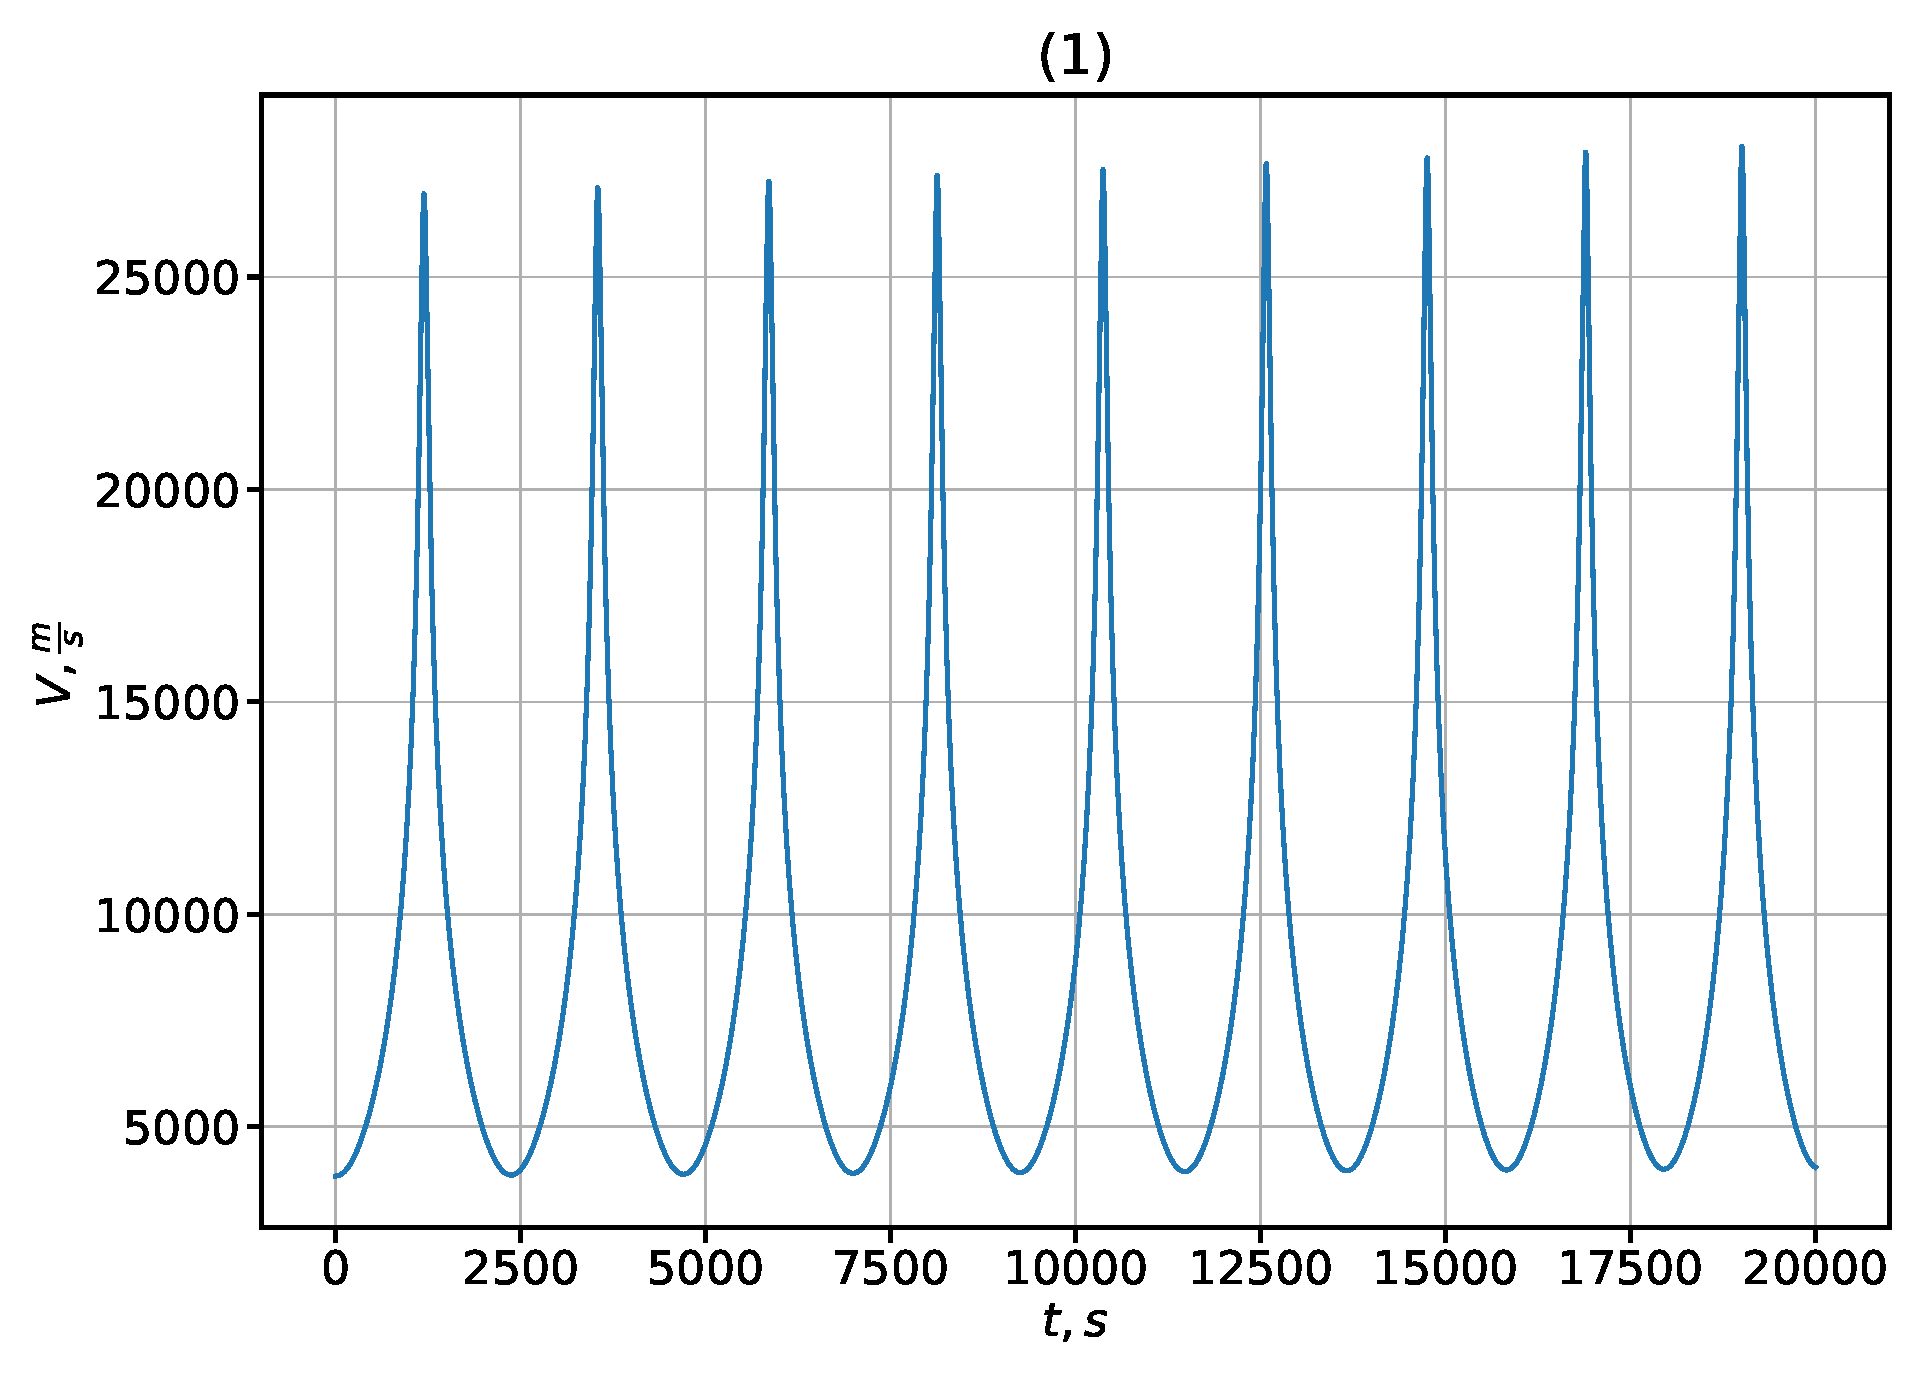
\includegraphics[width=1.0\linewidth]{V_t_1.eps}
    \endminipage\hfill
    \minipage{0.33\textwidth}
      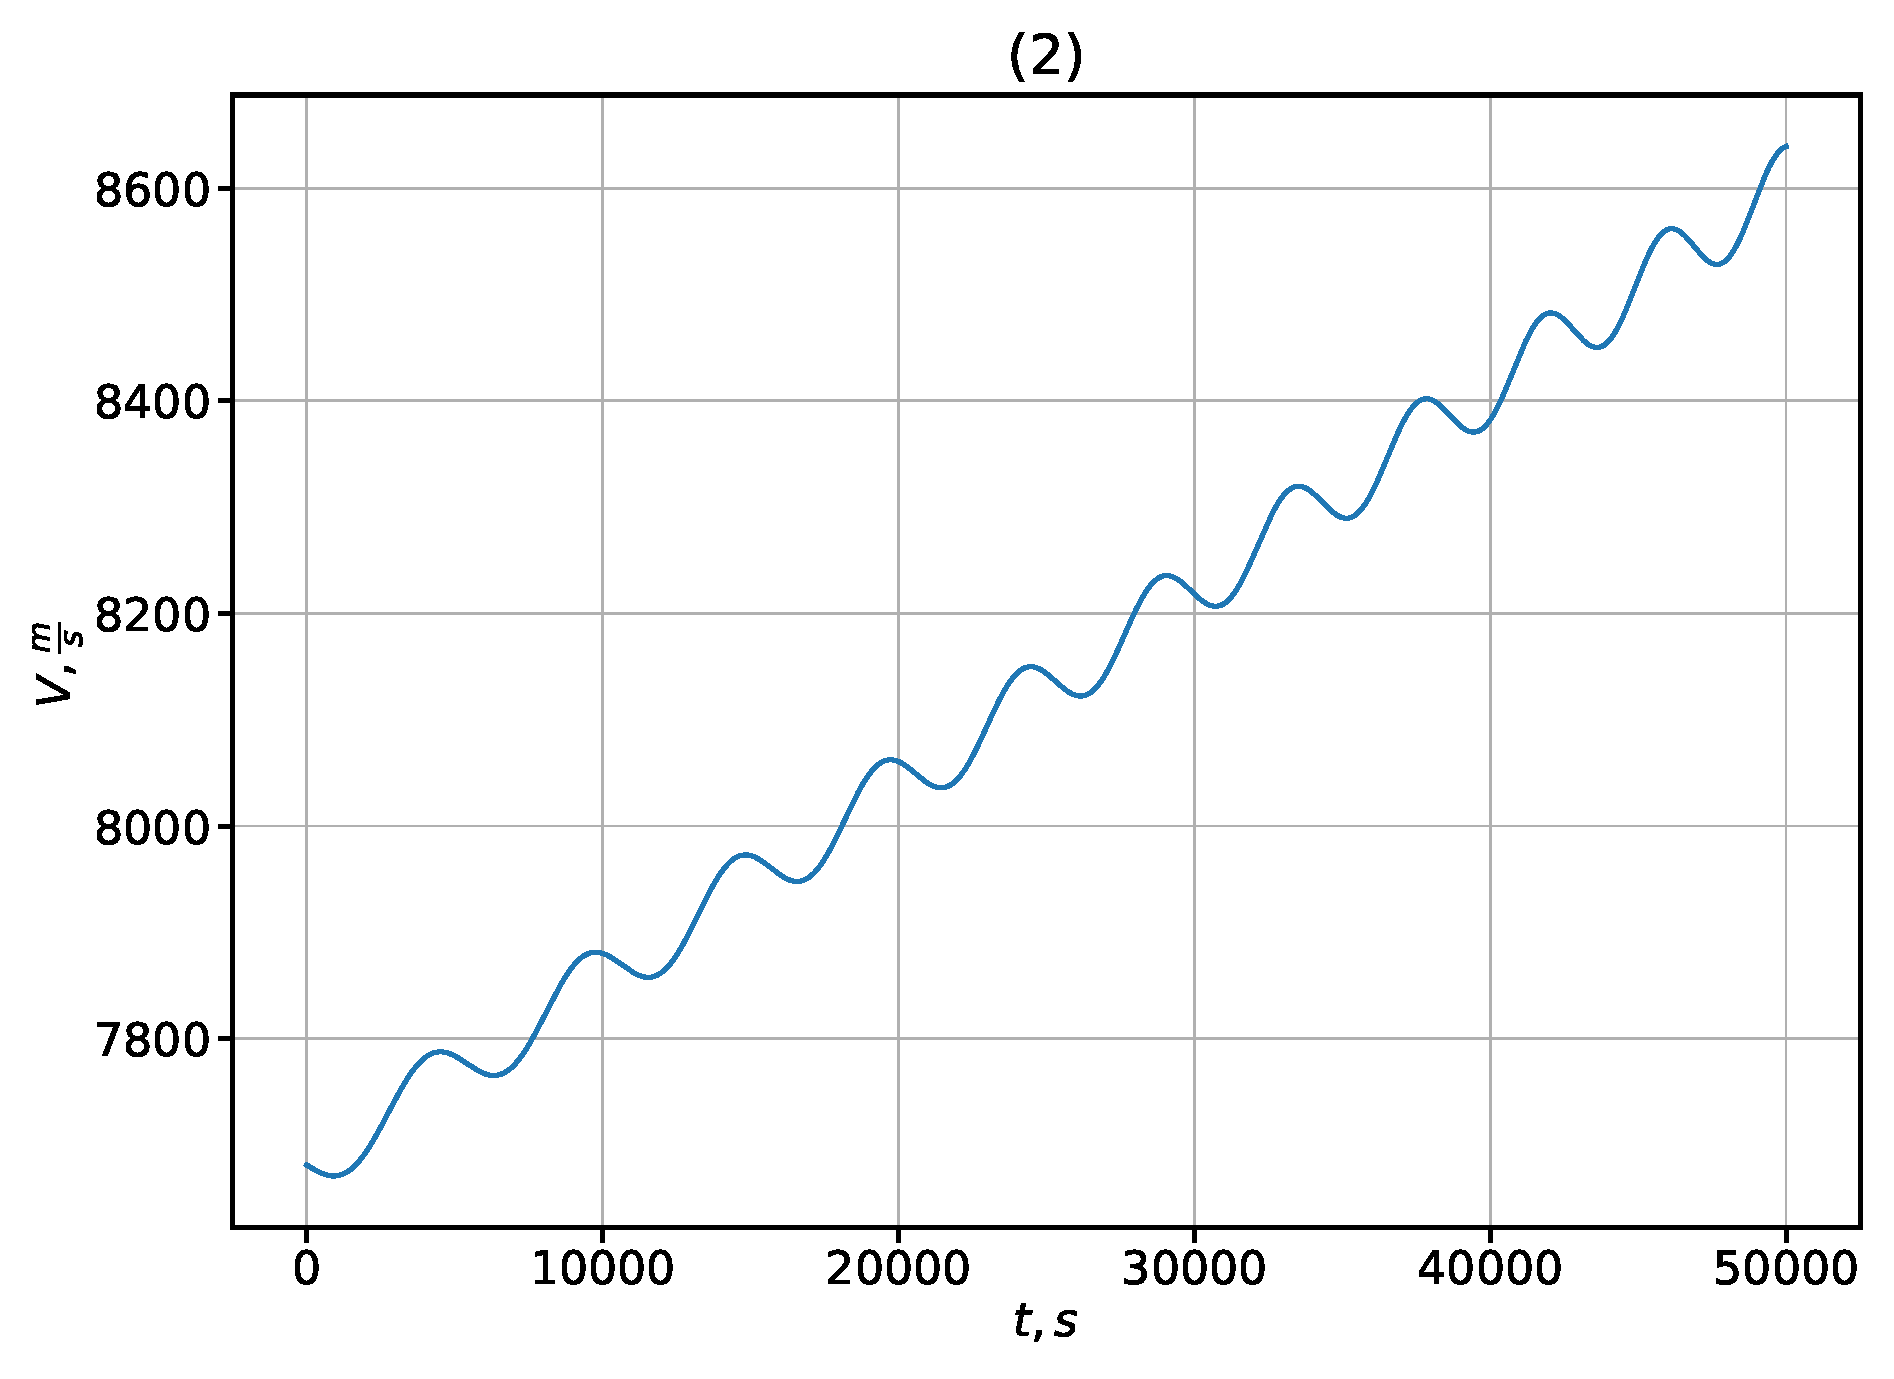
\includegraphics[width=1.0\linewidth]{V_t_2.eps}
    \endminipage\hfill
    \minipage{0.33\textwidth}
      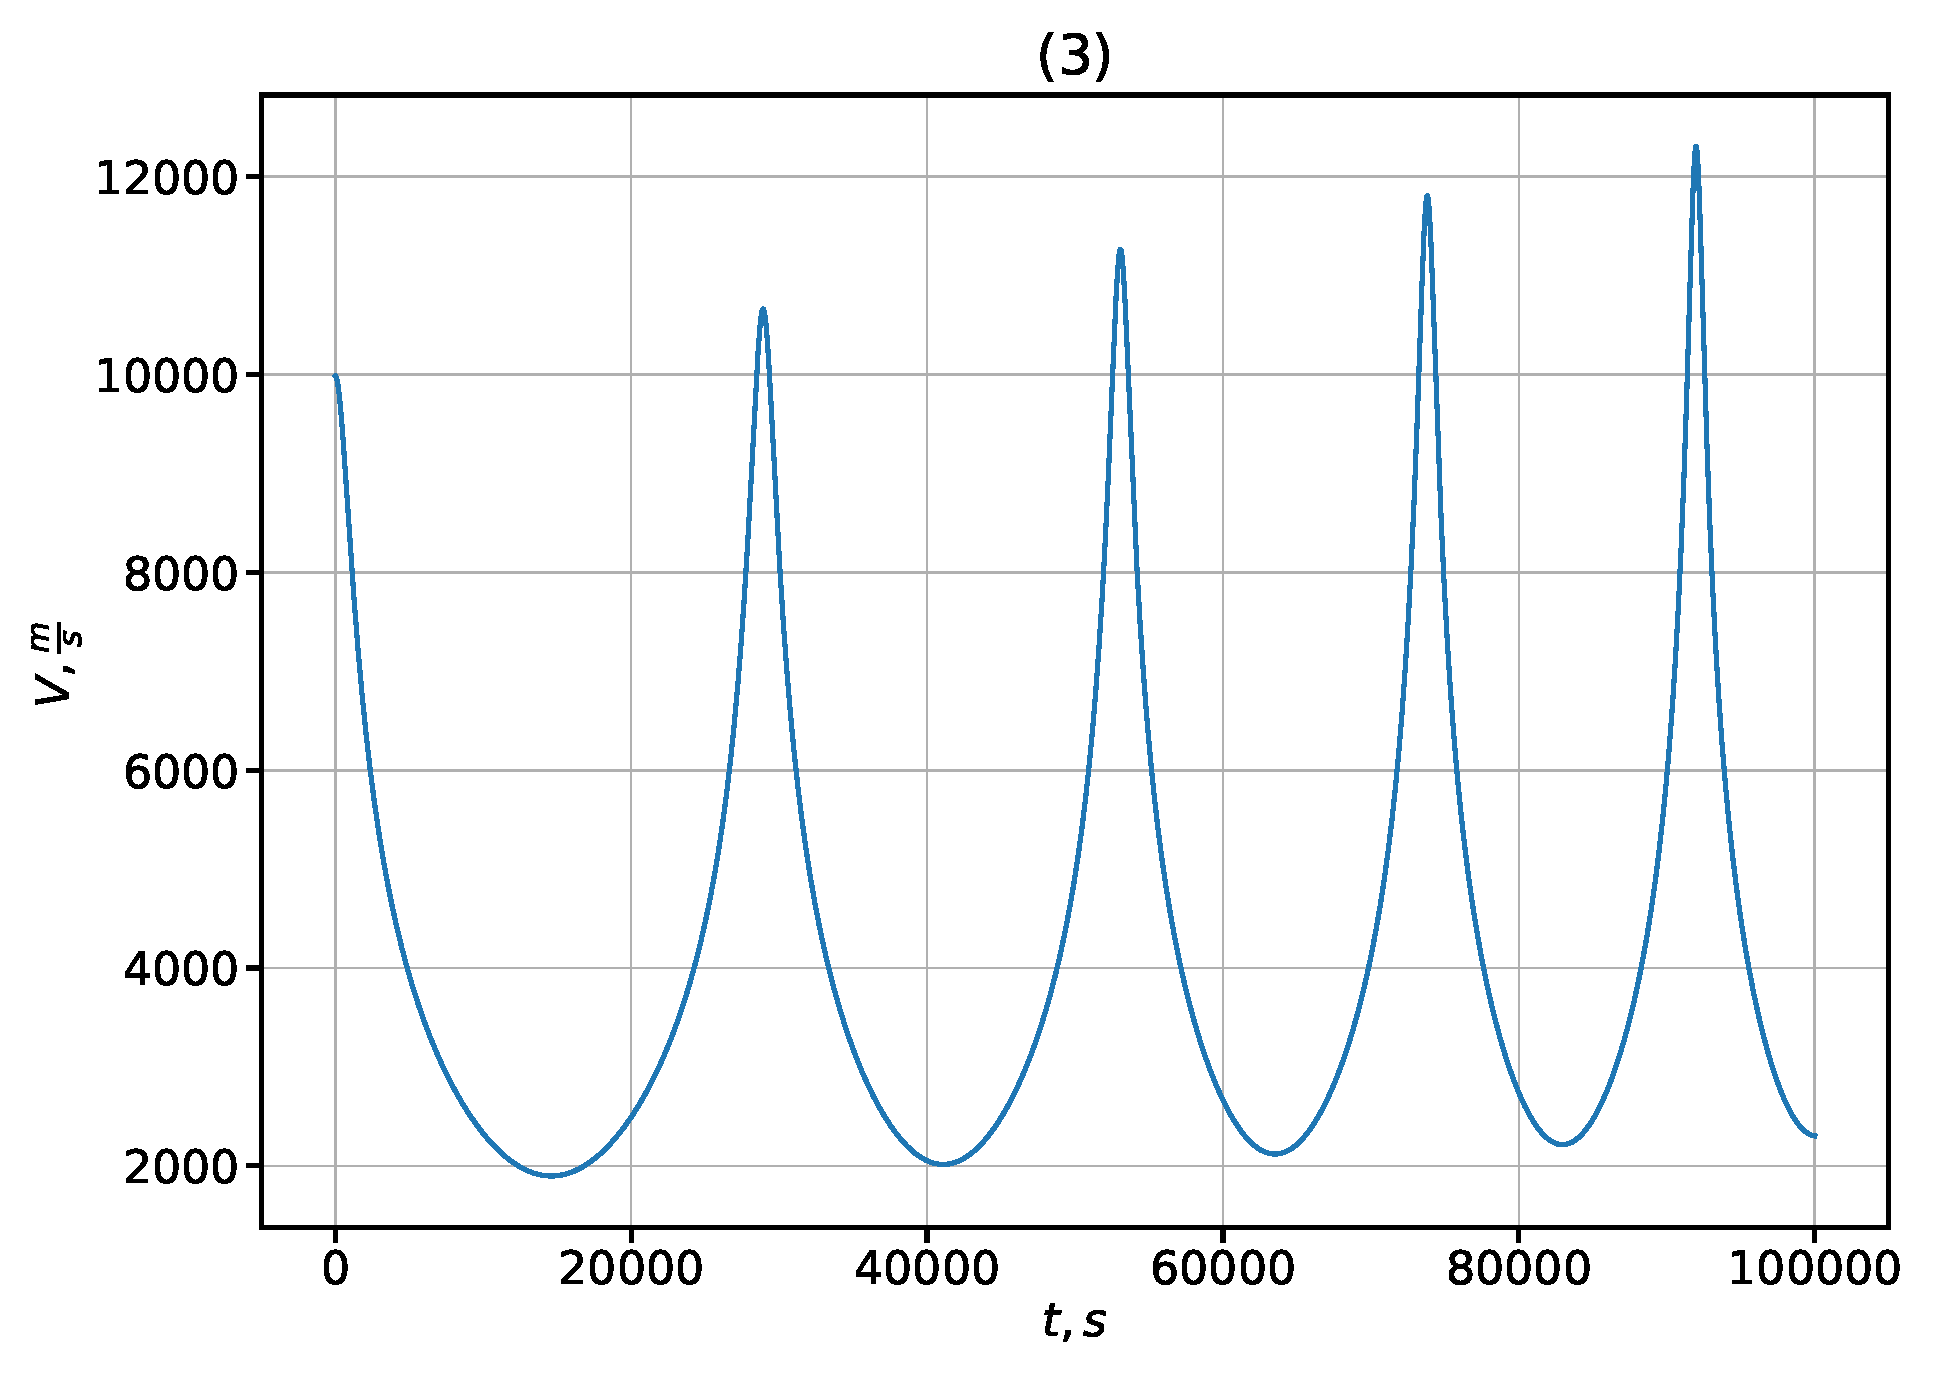
\includegraphics[width=1.0\linewidth]{V_t_3.eps}
    \endminipage
    \caption{Зависимости орбитальных скоростей тел $V$ от времени $t$.}
    \label{fig:2}
    \end{figure}

Приведём графики зависимостей расстояний до тел от времени (Рис. \ref{fig:3}). Построив на графиках кривые, оценивающие максимальное и минимальное
расстояние до тела (Выражения \ref{eq:10}, \ref{eq:11}), заметим, что за положение тела находится строго между рассчитанными значениями, что 
подтверждает правильность модели. В случае круговой орбиты рассчитанное значение фокального параметра является средним значением положения тела,
при этом не совпадает с ним в точности из-за наличия малой эллиптичности у орбиты, аналогично возмущениям скорости.
\begin{figure}[H]
    \minipage{0.33\textwidth}
      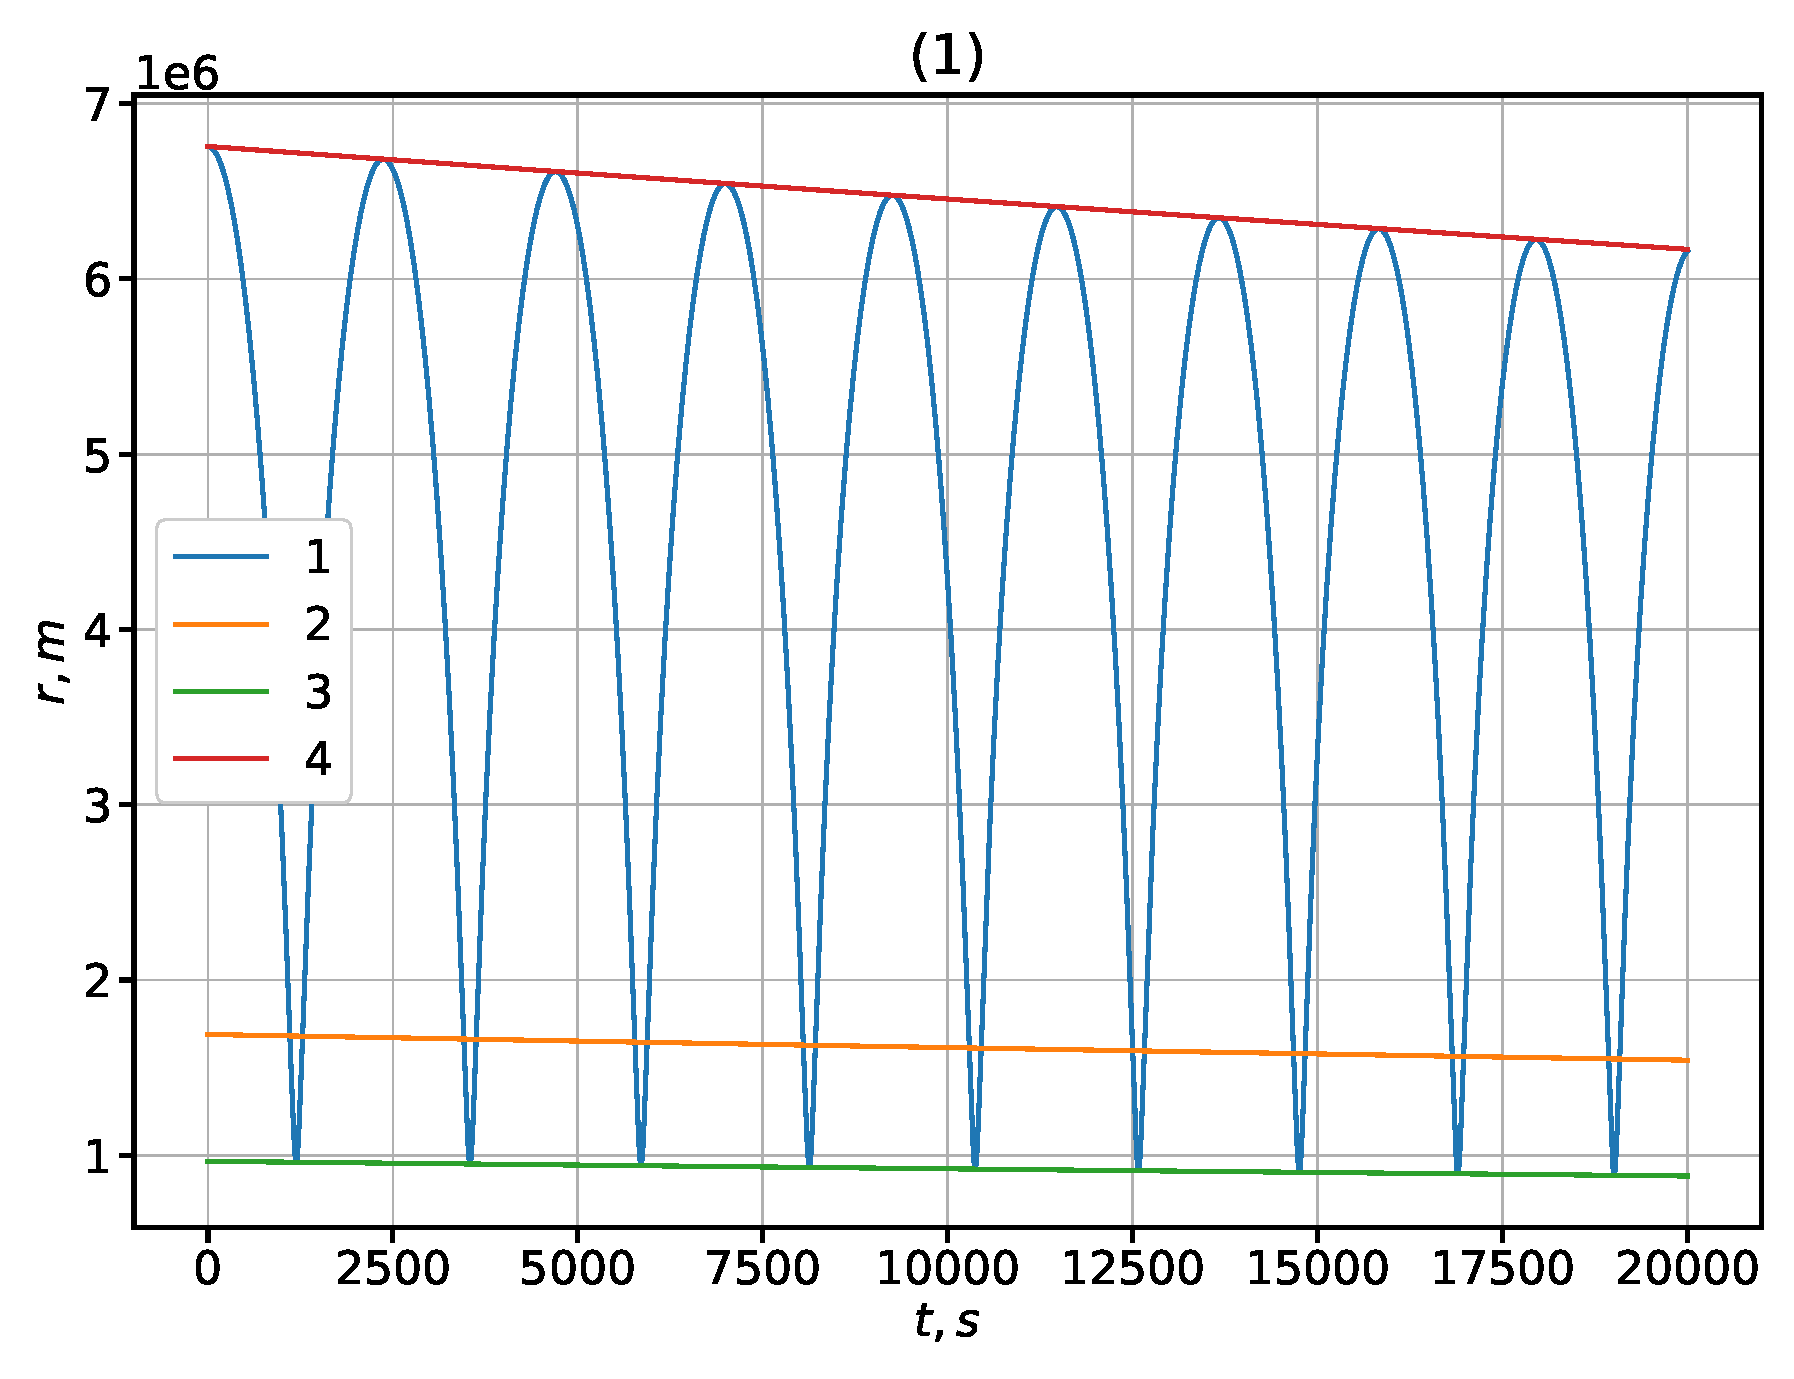
\includegraphics[width=1.0\linewidth]{r_t_1.eps}
    \endminipage\hfill
    \minipage{0.33\textwidth}
      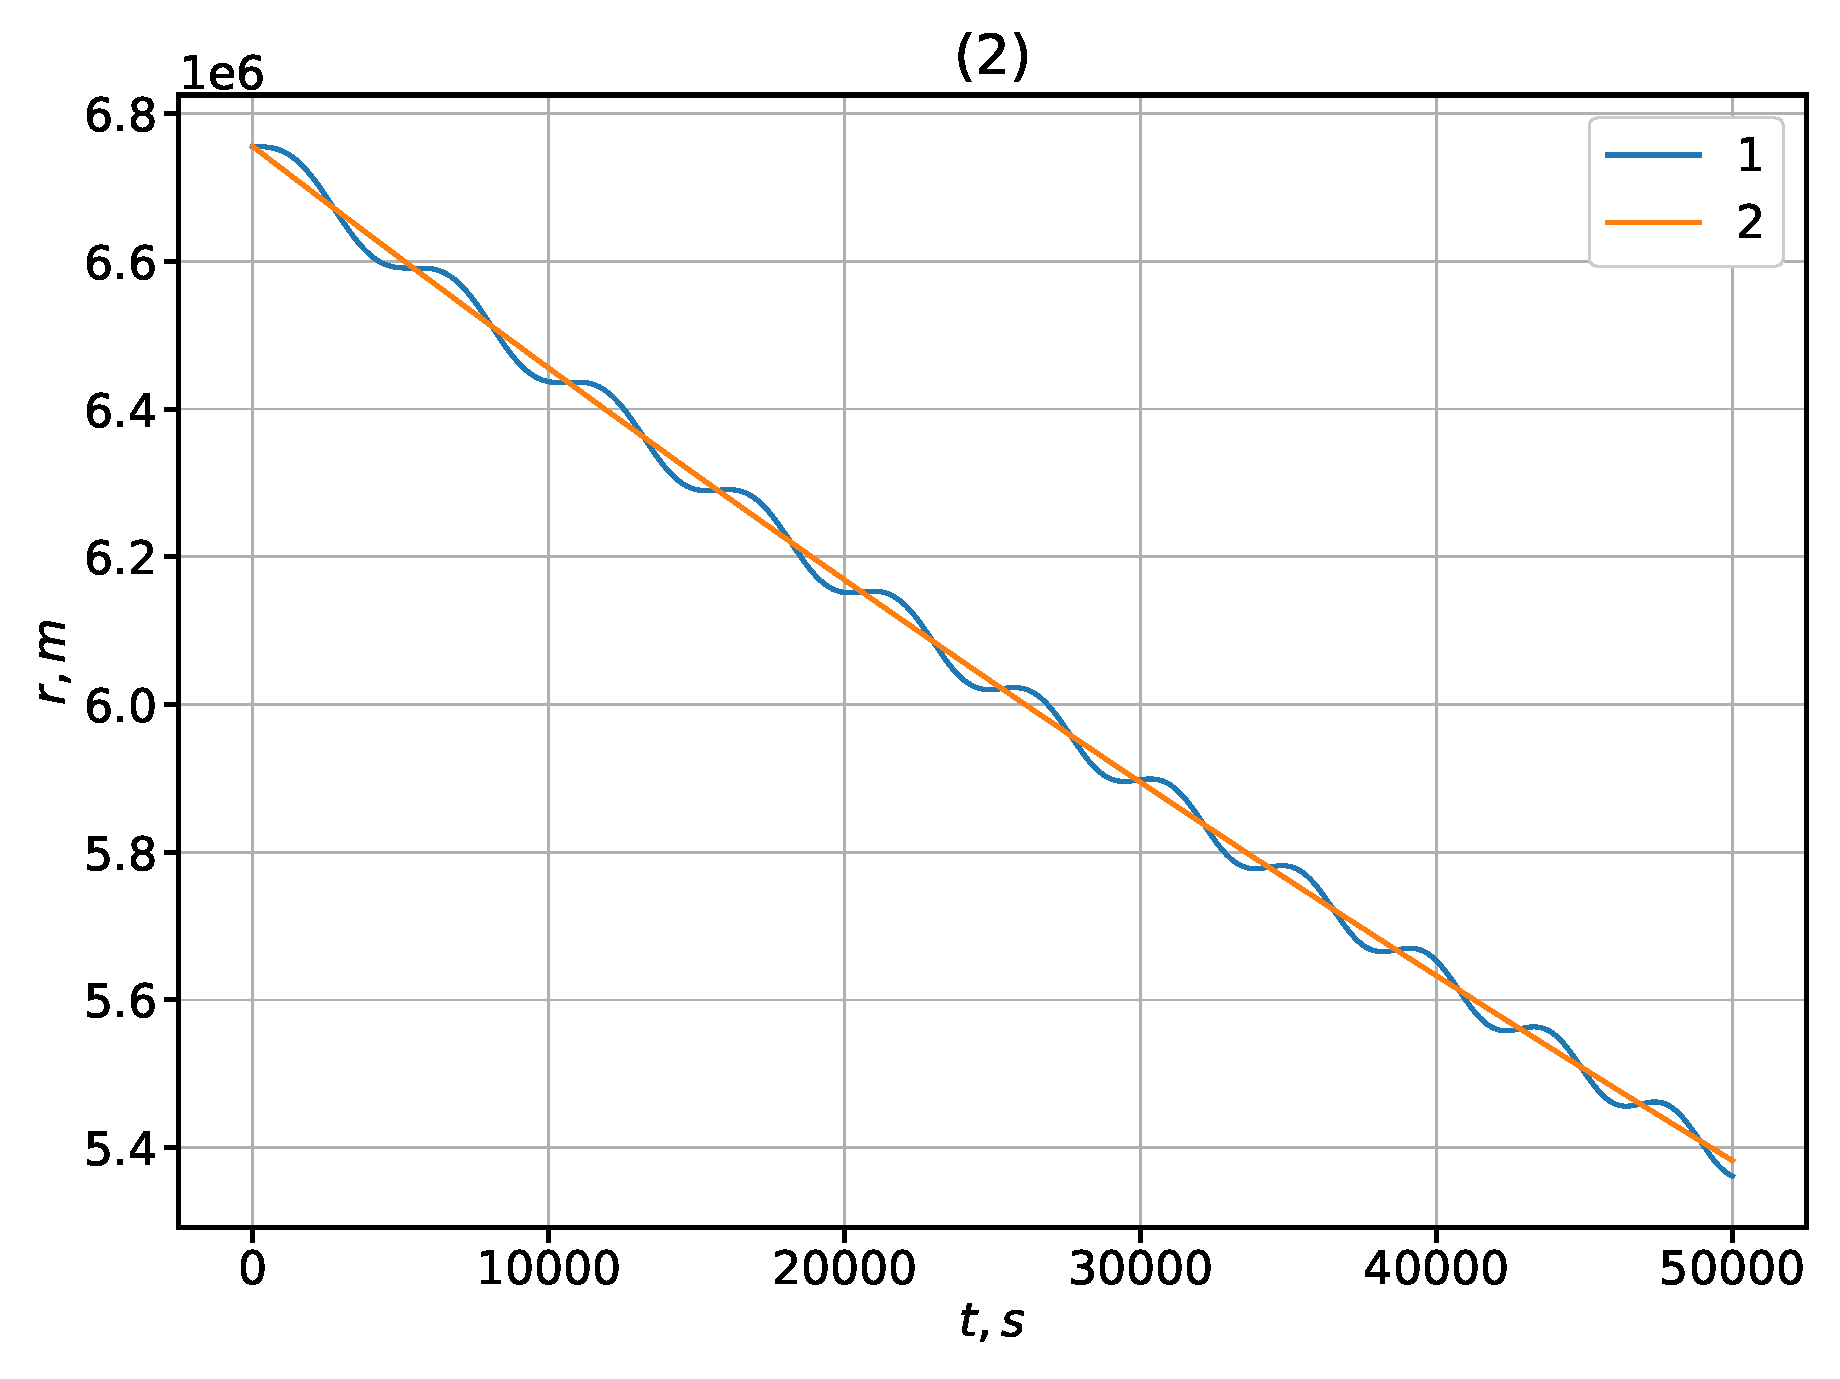
\includegraphics[width=1.0\linewidth]{r_t_2.eps}
    \endminipage\hfill
    \minipage{0.33\textwidth}
      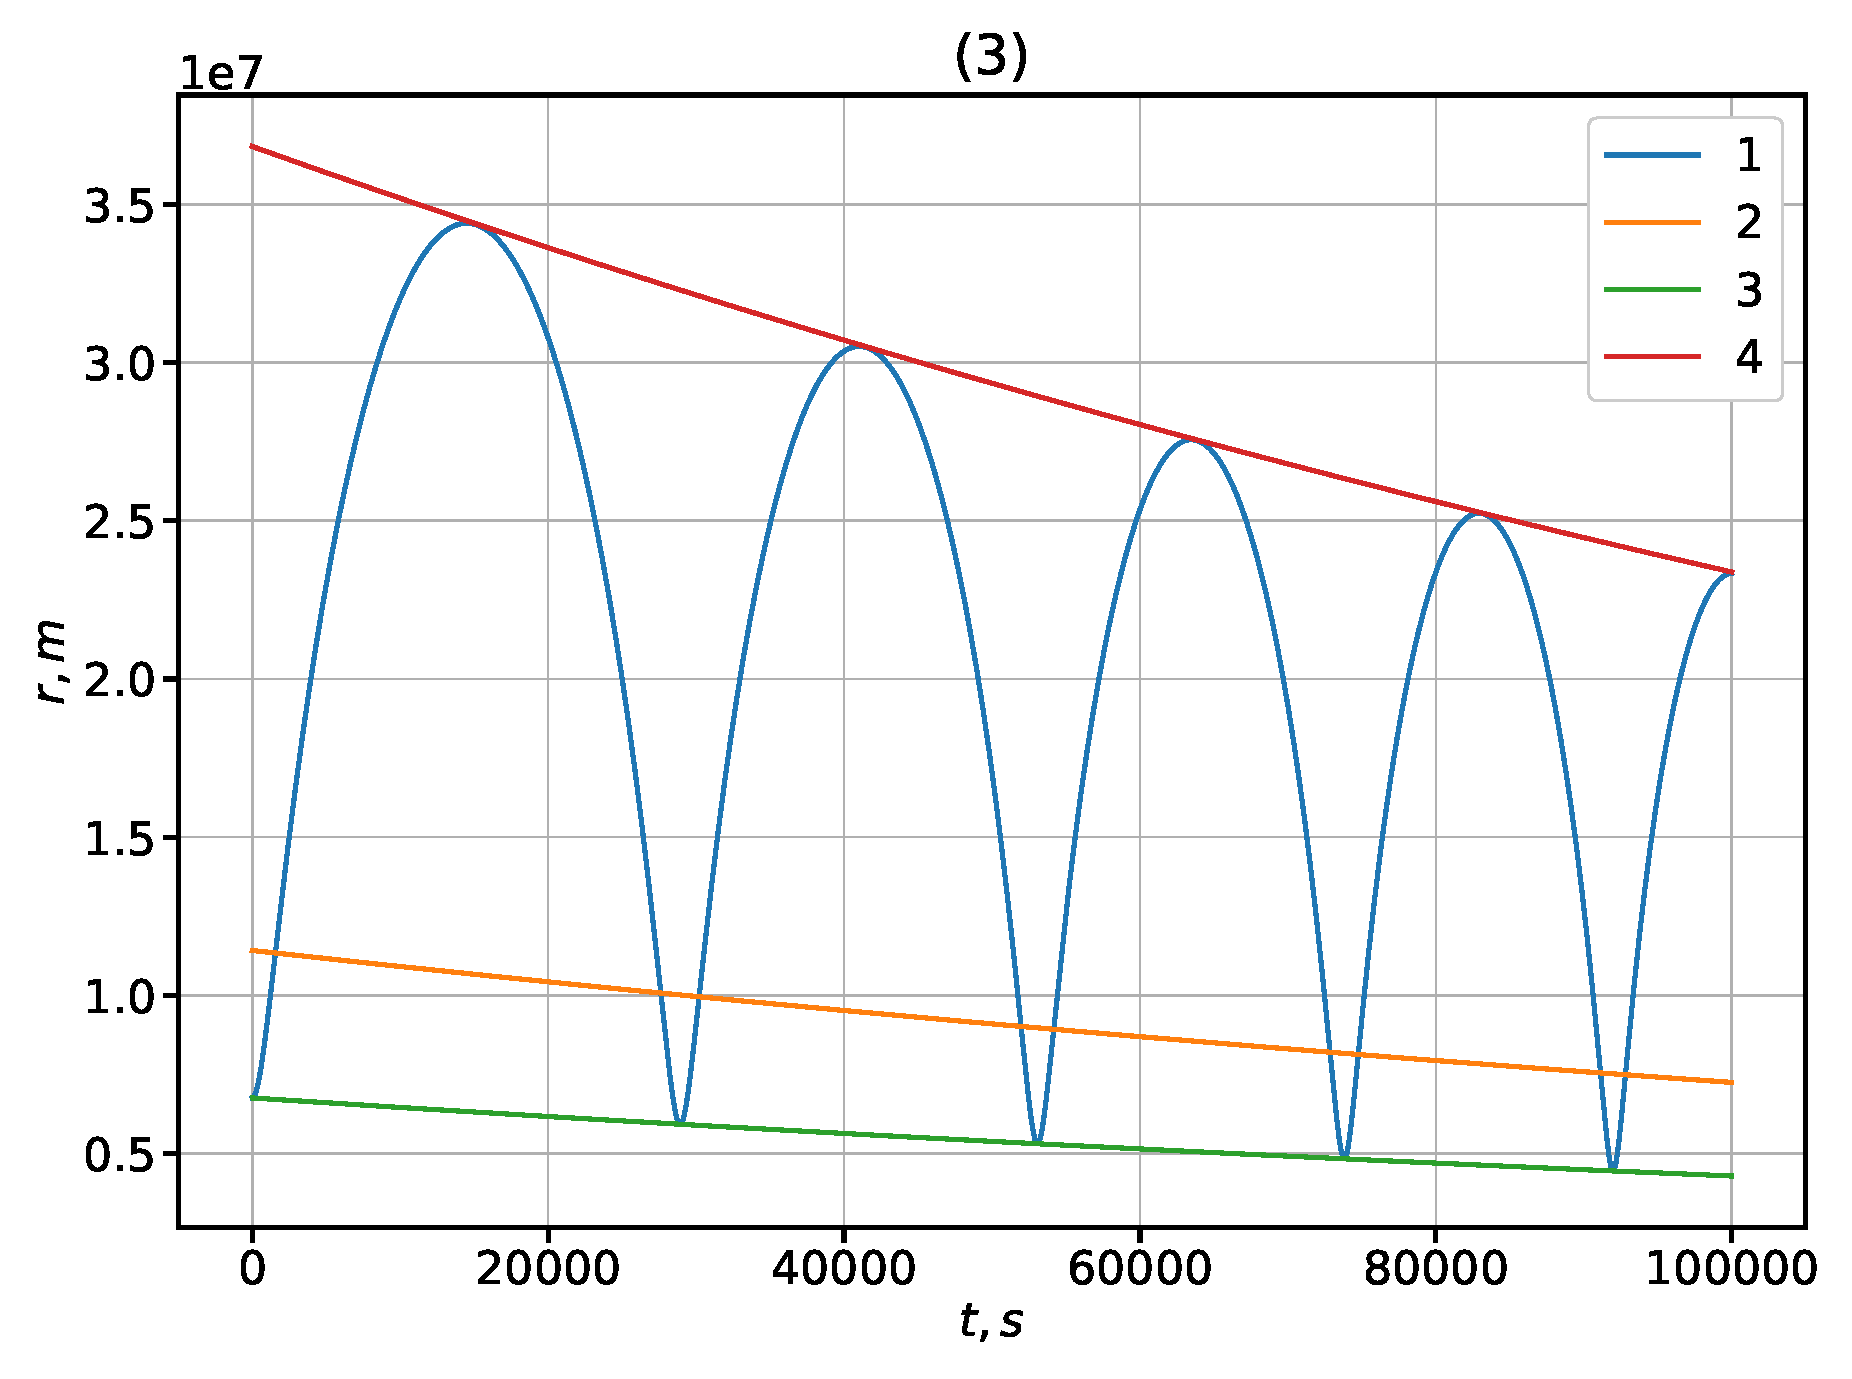
\includegraphics[width=1.0\linewidth]{r_t_3.eps}
    \endminipage
    \caption{Зависимости расстояний до тел от центра Земли $r$ от времени $t$. 1 - расстояние до тела, 
    2 - рассчитанное значение фокального параметра орбиты (Выражение \ref{eq:9}), 3 - минимально возможное положения тела (Выражение \ref{eq:11}), 
    4 - максимально возможное положения тела (Выражение \ref{eq:10}).}
    \label{fig:3}
    \end{figure}
Из графиков (Рис. \ref{fig:4}) следует точное совпадения предсказанного значения момента импульса (Выражение \ref{eq:3})  с рассчитанными численно.
\begin{figure}[H]
    \minipage{0.33\textwidth}
      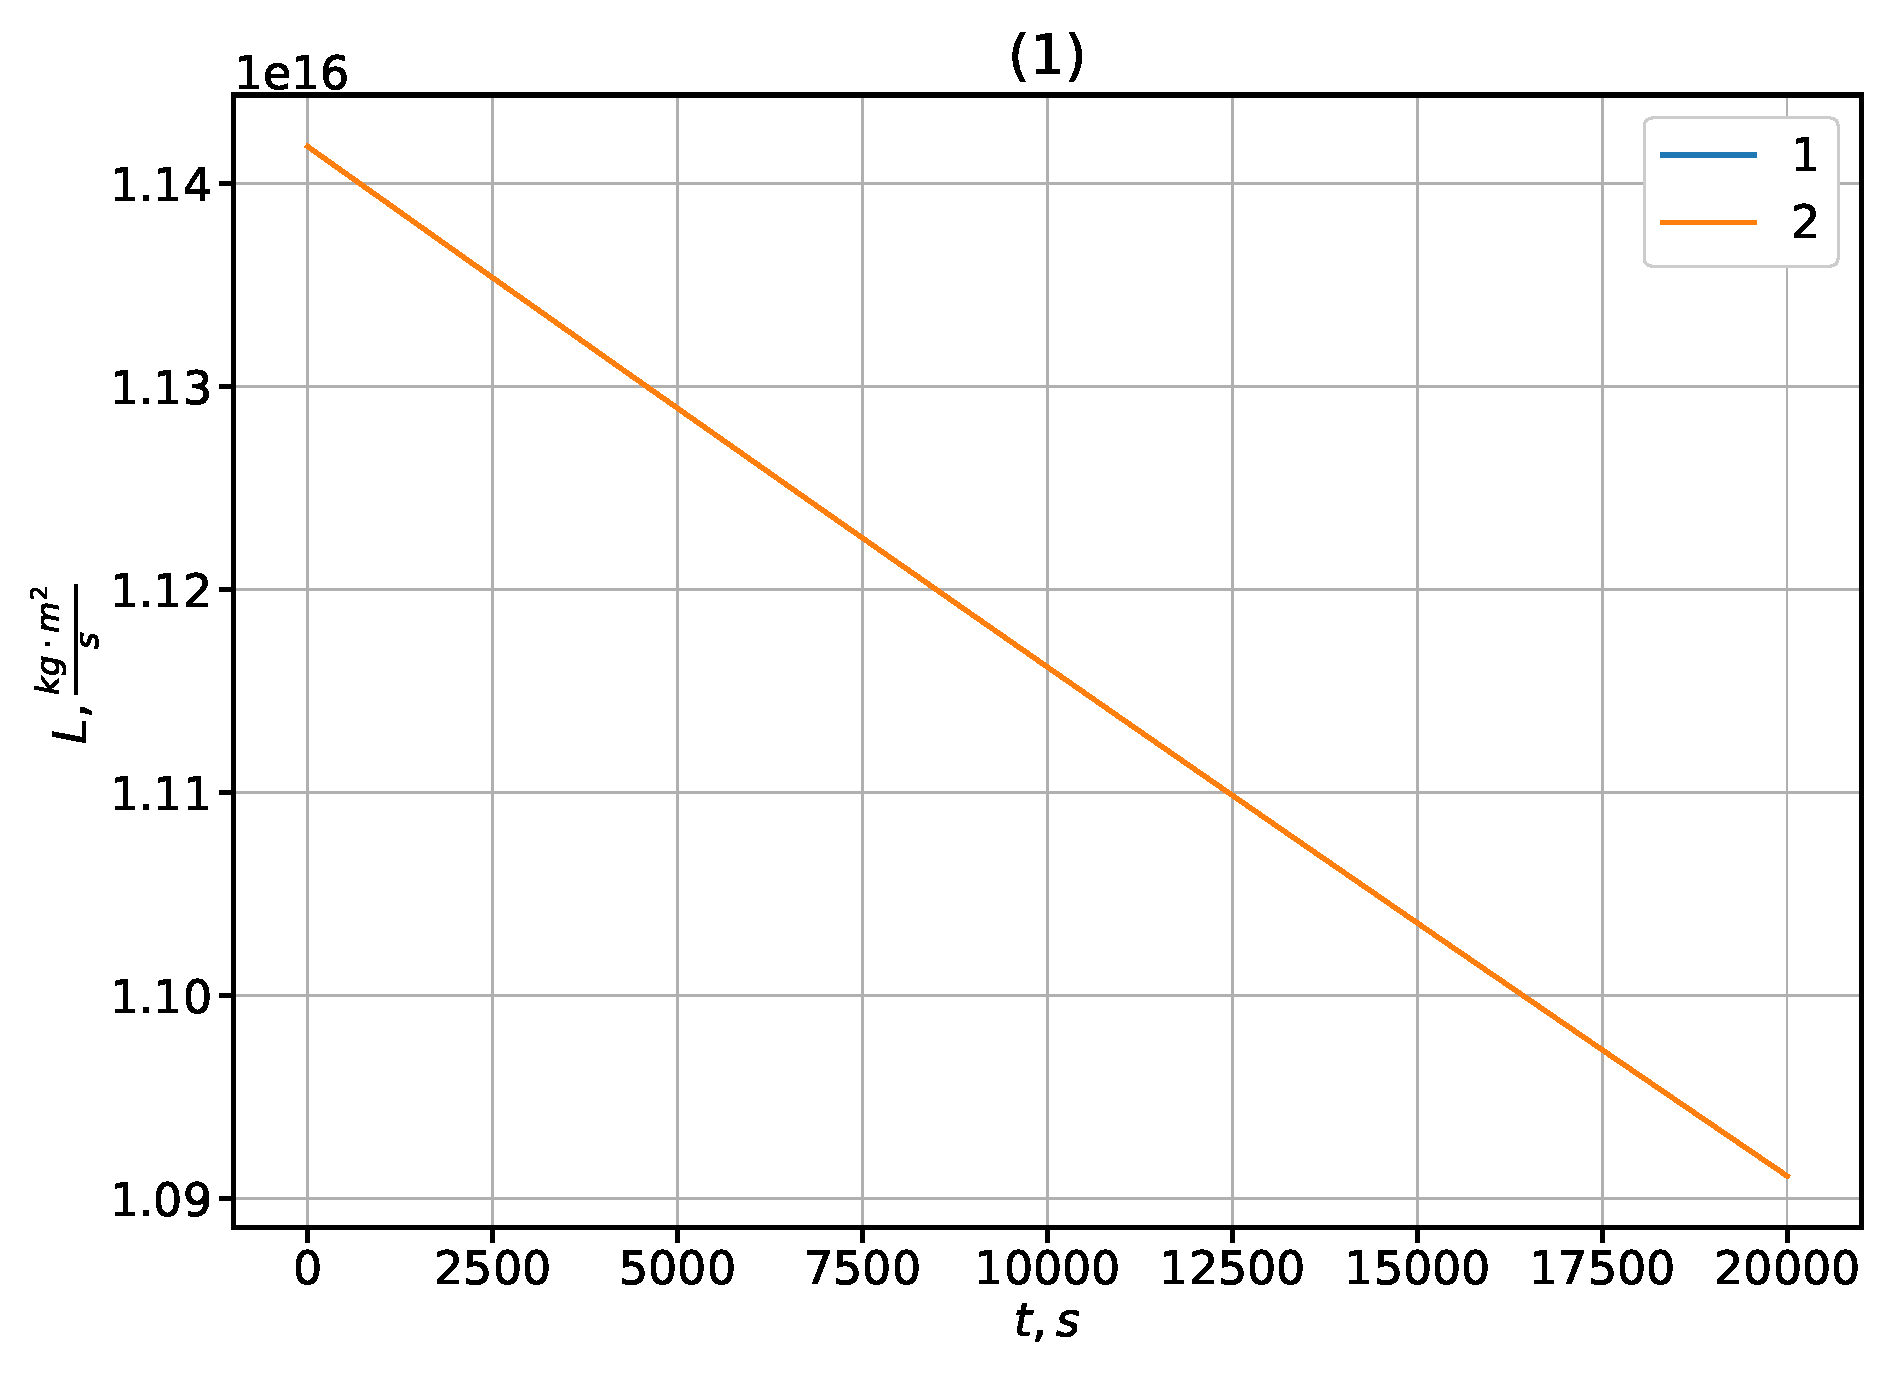
\includegraphics[width=1.0\linewidth]{L_t_1.eps}
    \endminipage\hfill
    \minipage{0.33\textwidth}
      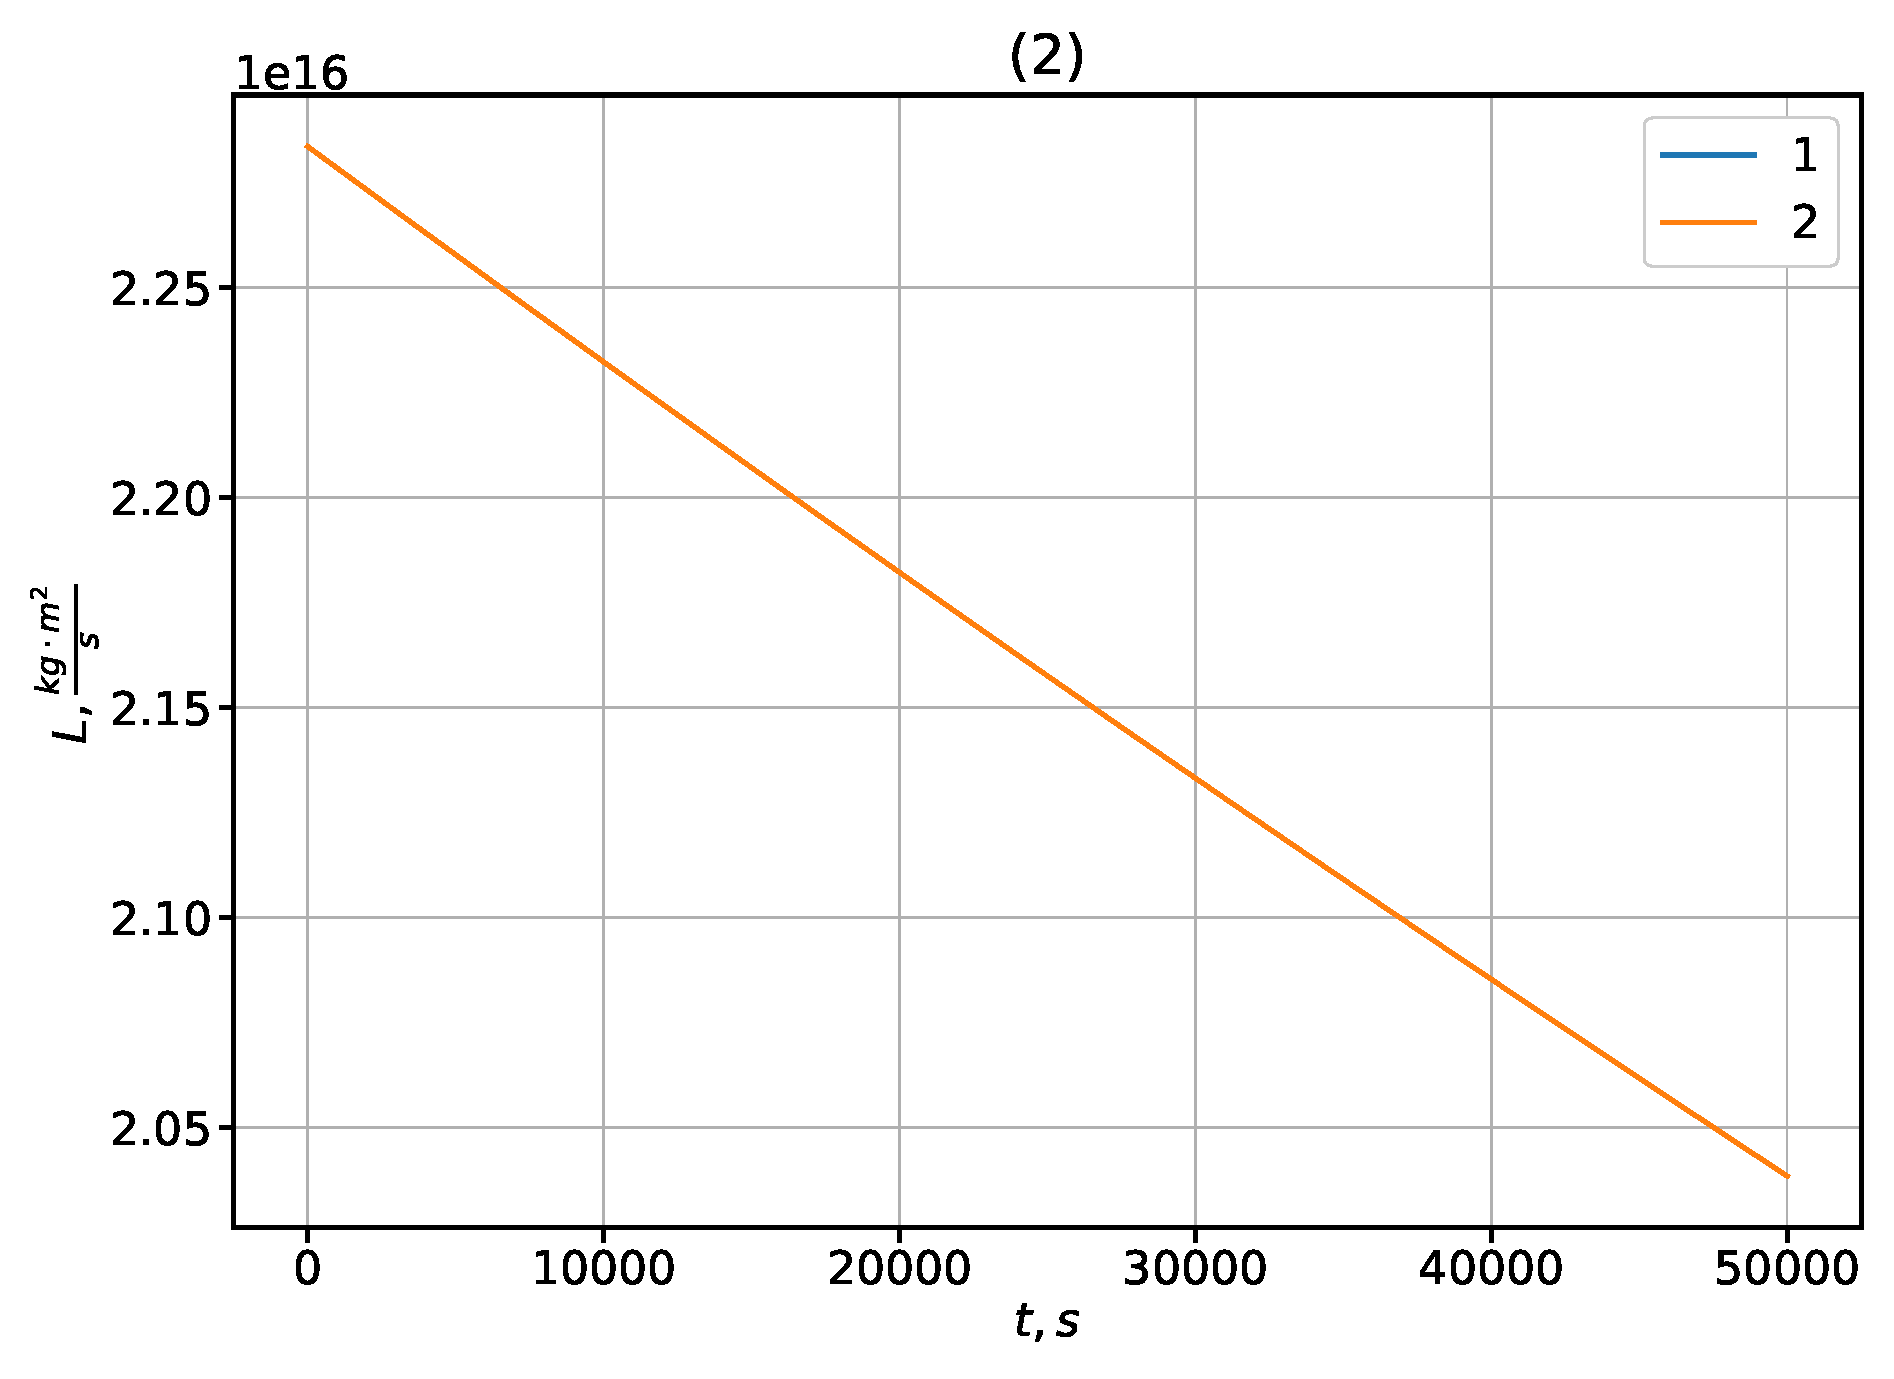
\includegraphics[width=1.0\linewidth]{L_t_2.eps}
    \endminipage\hfill
    \minipage{0.33\textwidth}
      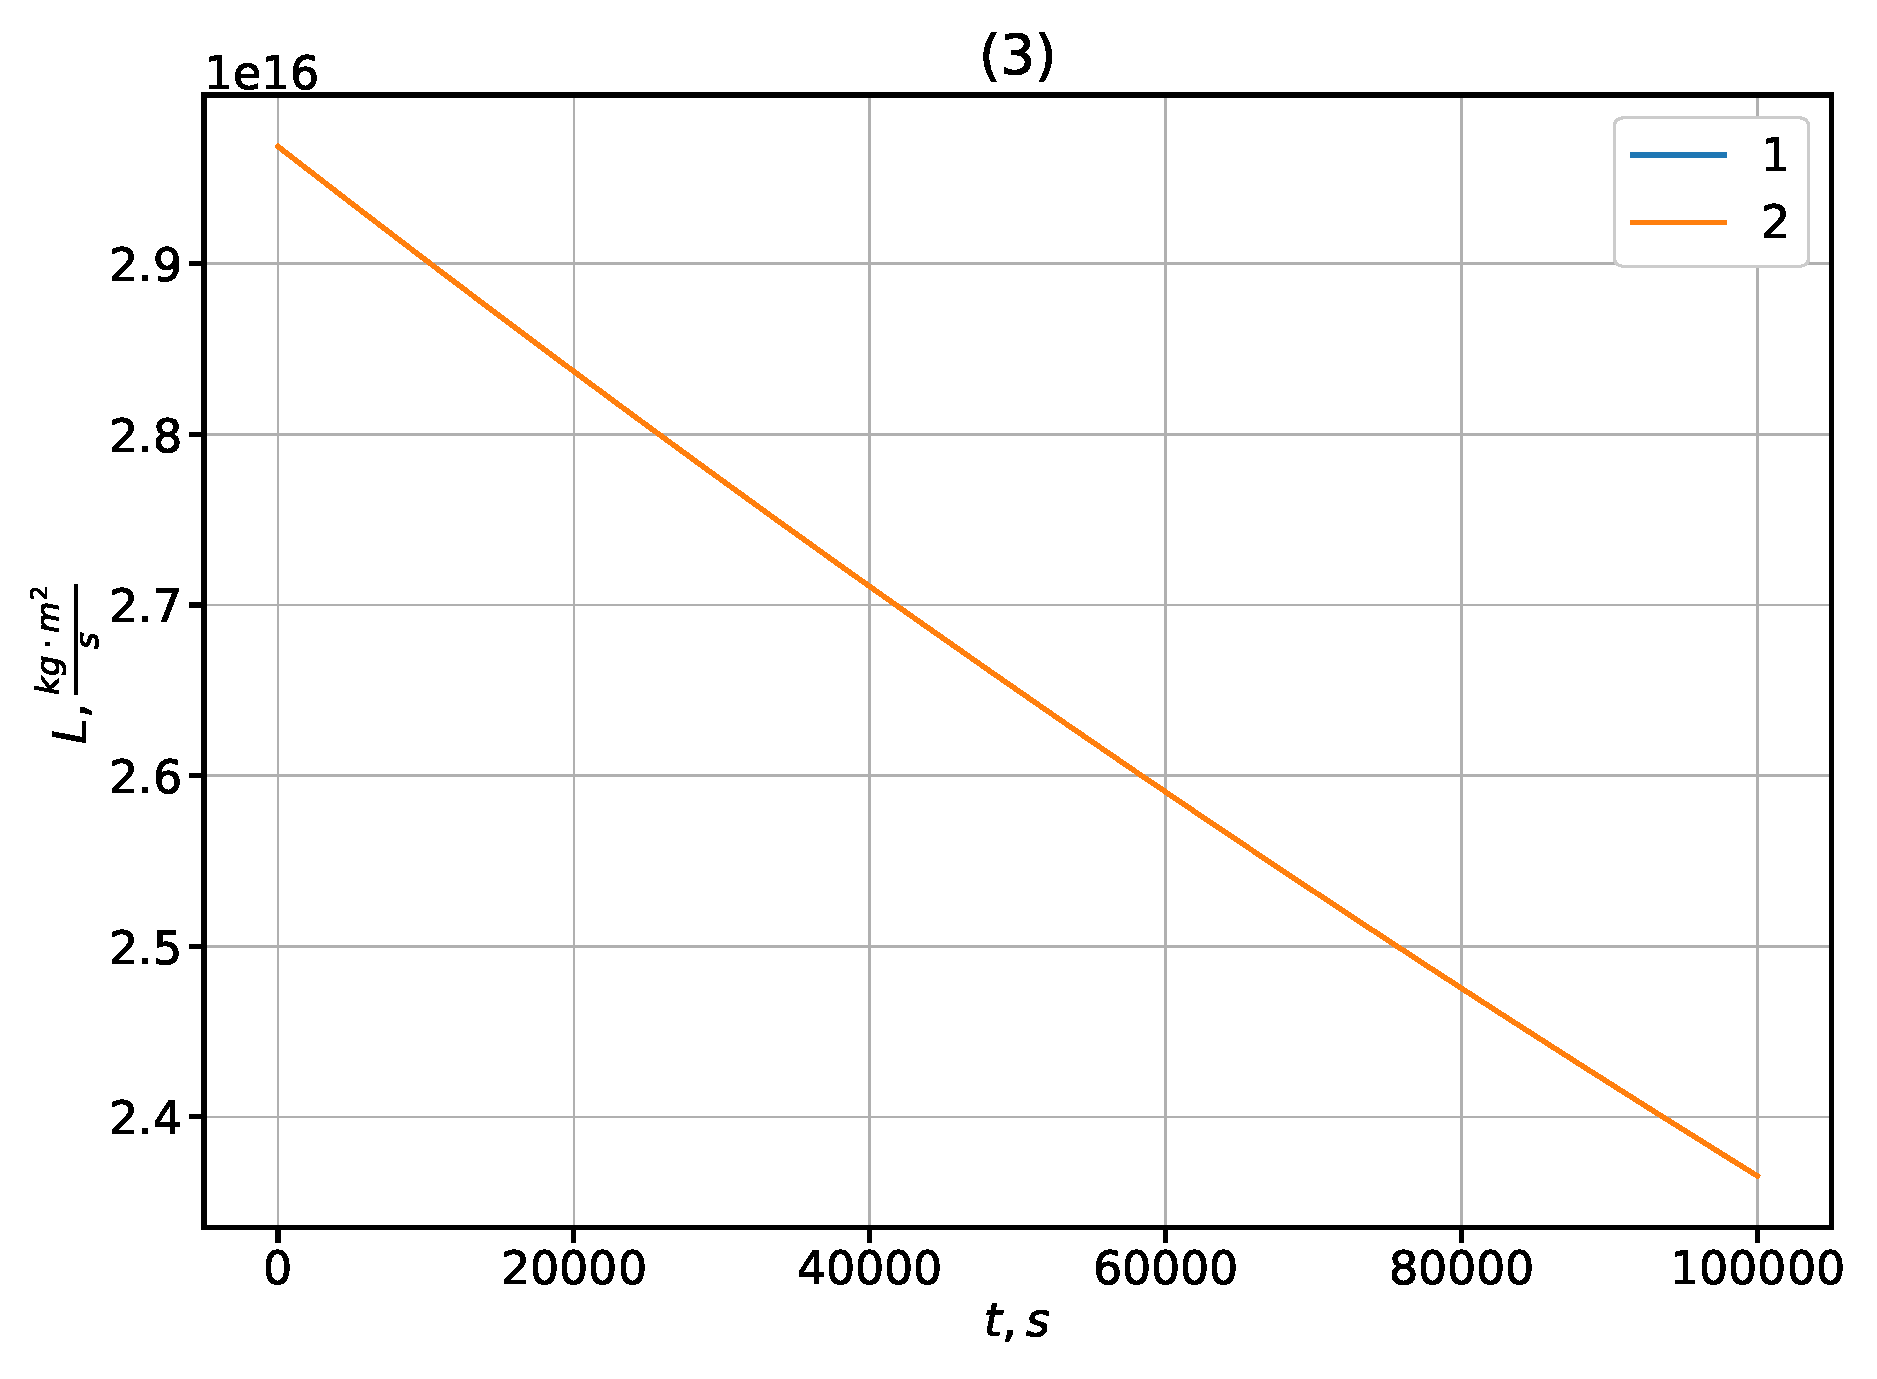
\includegraphics[width=1.0\linewidth]{L_t_3.eps}
    \endminipage
    \caption{Зависимости моментов импульса тел $L$ от времени $t$. 1 - численно рассчитанный момент импульса, 
    2 - предсказанный момент имульса (Выражение \ref{eq:3}).}
    \label{fig:4}
    \end{figure}

Приведём графики зависимости полной энергии тела от времени (Рис. \ref{fig:5}). Во всех симуляциях среднее значение энергии за любой из периодов
совпала с рассчитанной (Выражение \ref{eq:7}). В случае круговой орбиты полная энергия тела почти не отличается от среднего значения, это происходит
из-за условного постоянства кинетической энергии тела, тогда отношение \ref{eq:5} выполняется в каждый момент времени и выражение для средней полной
энергии тела \ref{eq:7} можно переписать для энергии тела в любой момент времени.
\begin{figure}[H]
    \minipage{0.33\textwidth}
      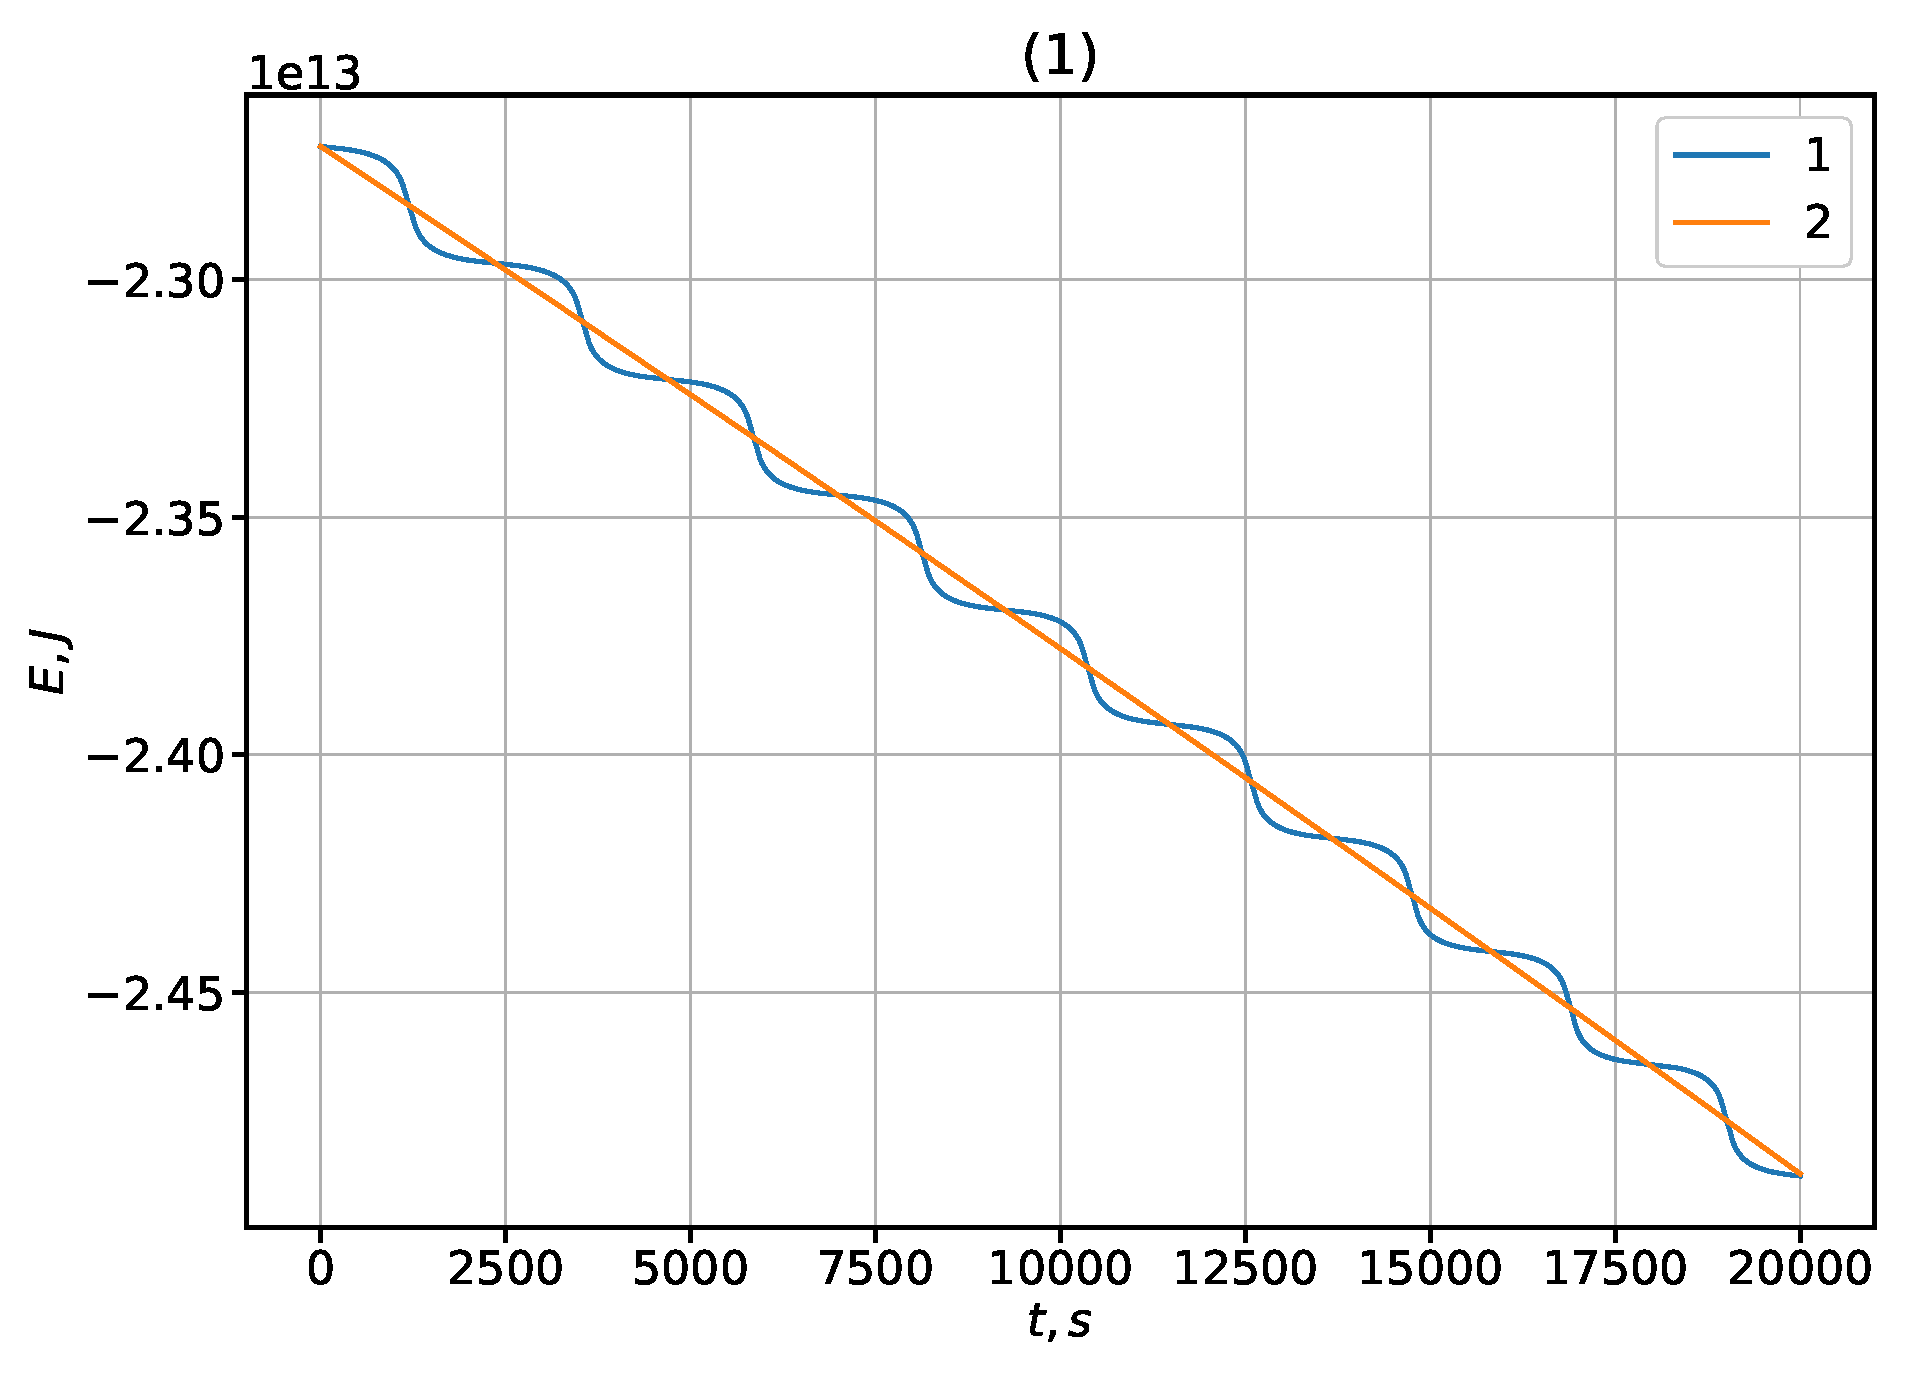
\includegraphics[width=1.0\linewidth]{En_t_1.eps}
    \endminipage\hfill
    \minipage{0.33\textwidth}
      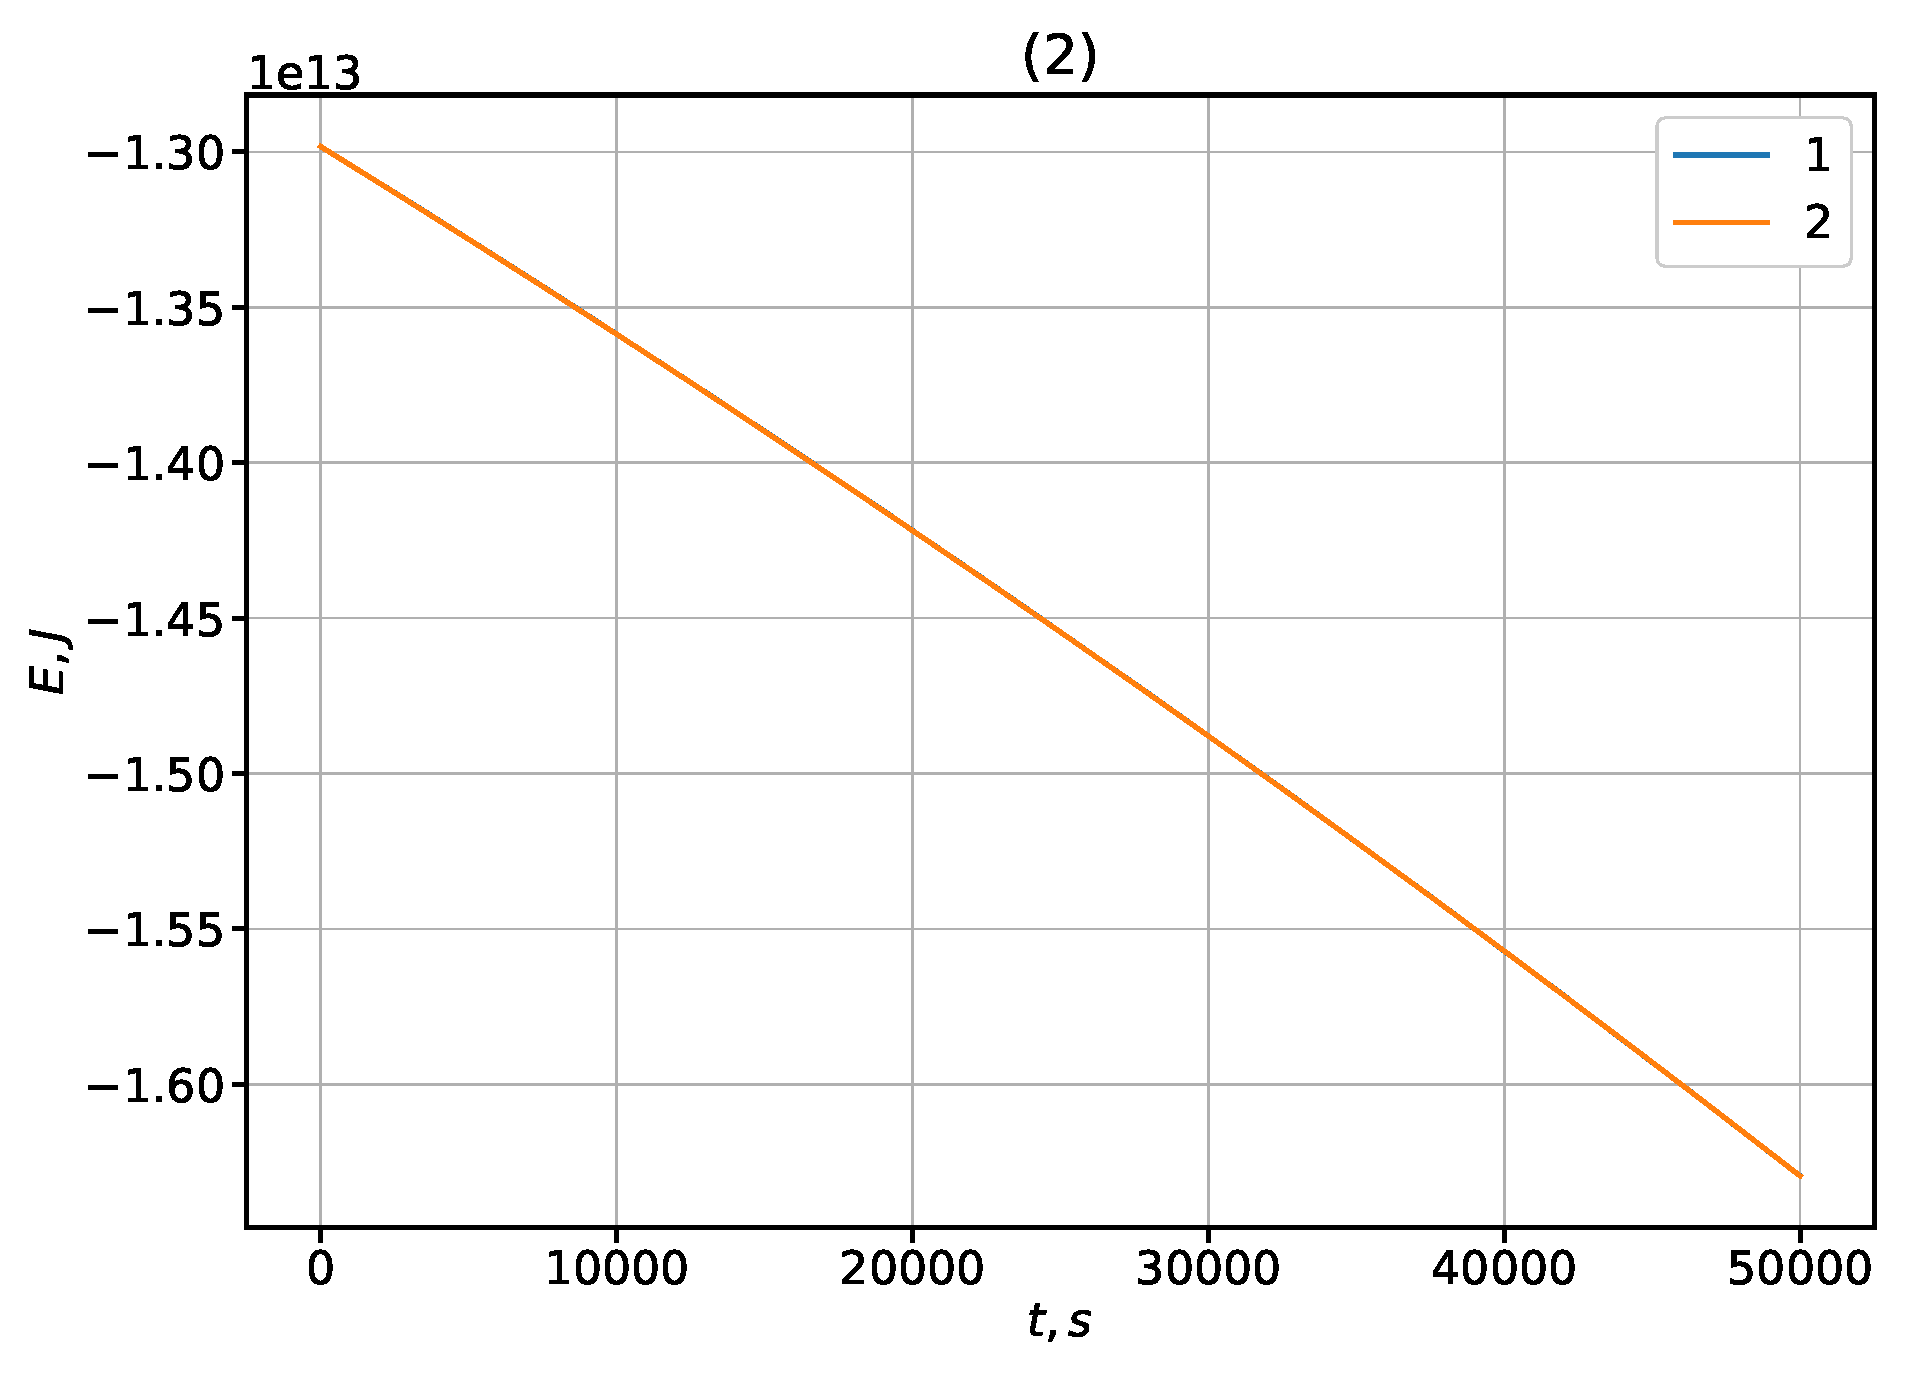
\includegraphics[width=1.0\linewidth]{En_t_2.eps}
    \endminipage\hfill
    \minipage{0.33\textwidth}
      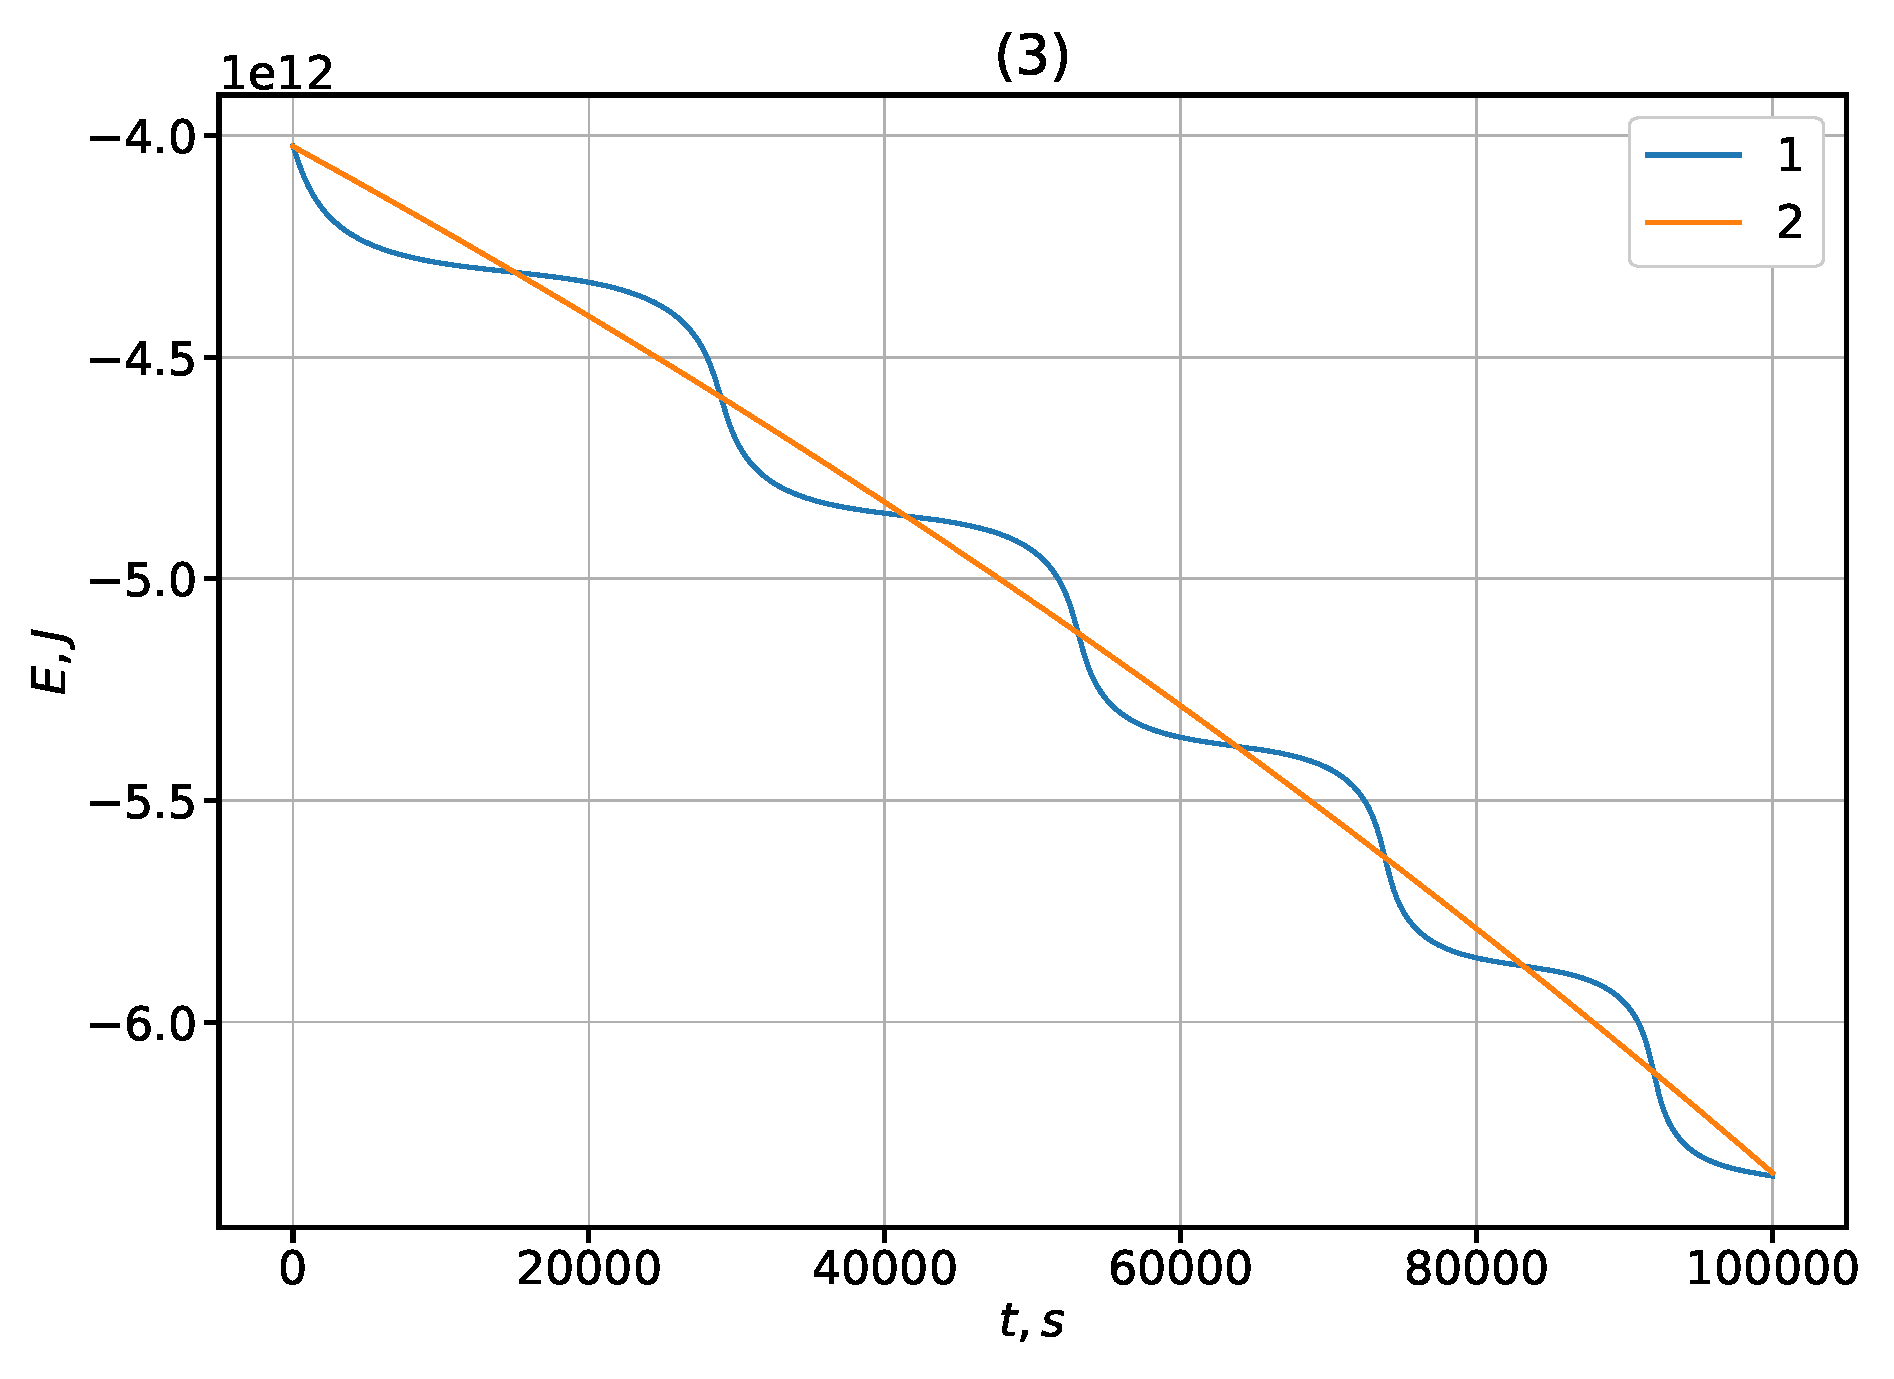
\includegraphics[width=1.0\linewidth]{En_t_3.eps}
    \endminipage
    \caption{Зависимости полной энергии тел $E$ от времени $t$. 1 - численно рассчитанная энергия тела, 
    2 - предсказанная средняя за период полная энергия тела (Выражени \ref{eq:7}).}
    \label{fig:5}
    \end{figure}
Рассмотрим графики значения эксцентреситета от времени (Рис. \ref{fig:6}). В первой и третьей симуляции значение эксцентреситета колеблется 
около начального значения, причём отклонения от начального значения не превосходят $2\%$, что предсказывалось выражением \ref{eq:8}. 
Во второй симуляции значение эксцентреситета колеблется около значения $0.004$, что подтверждает наличие небольшой добавочной эллиптичности.
Также из графиков следует, что с течением времени минимальные и максимальные значения эксцентреситета за период приближаются к среднему значению. 
\begin{figure}[H]
    \minipage{0.33\textwidth}
      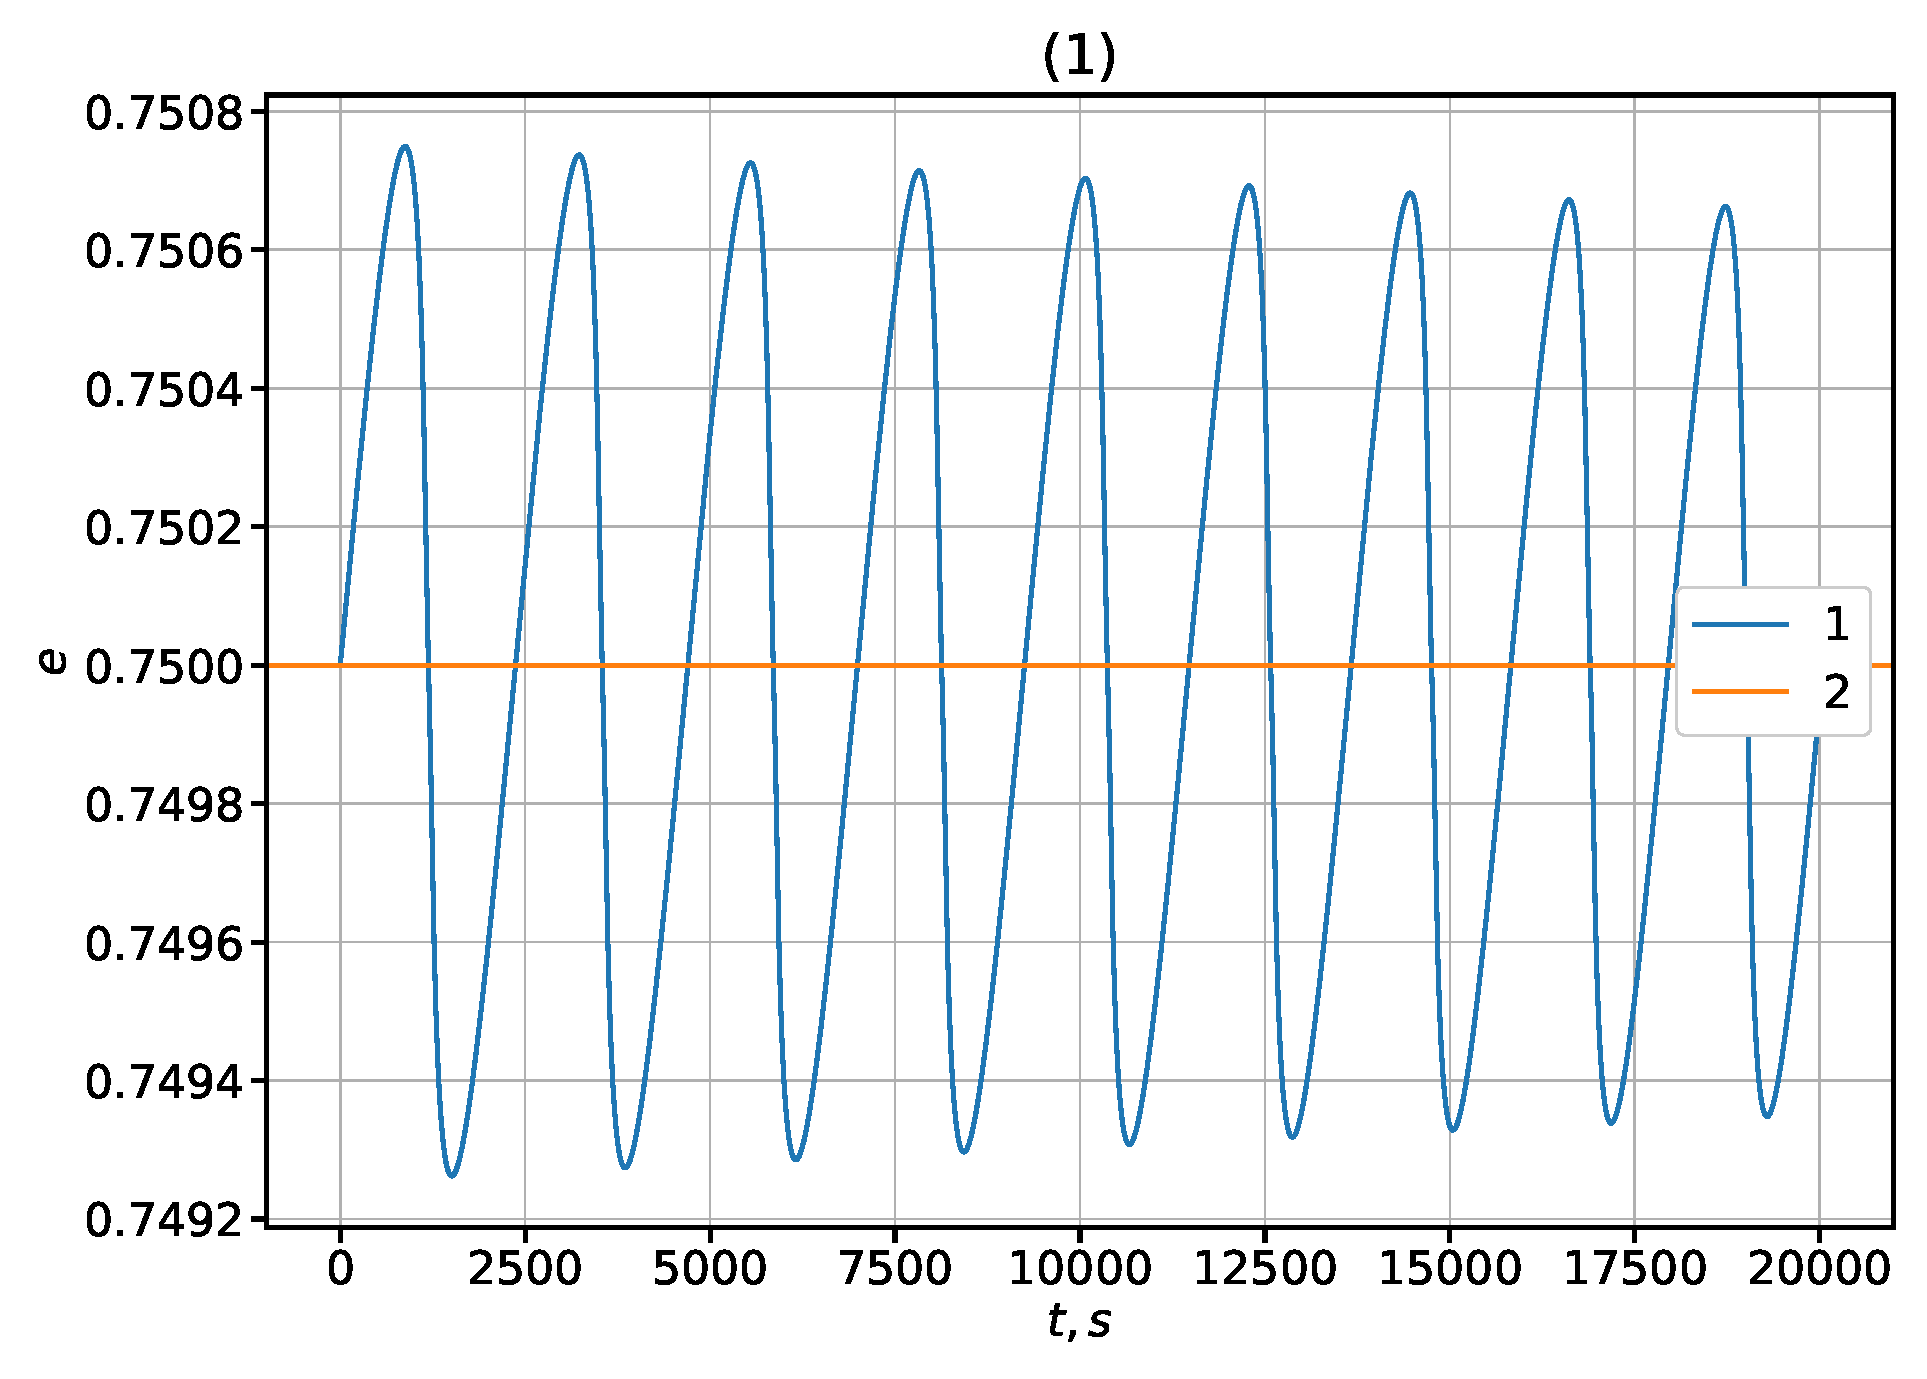
\includegraphics[width=1.0\linewidth]{e_t_1.eps}
    \endminipage\hfill
    \minipage{0.33\textwidth}
      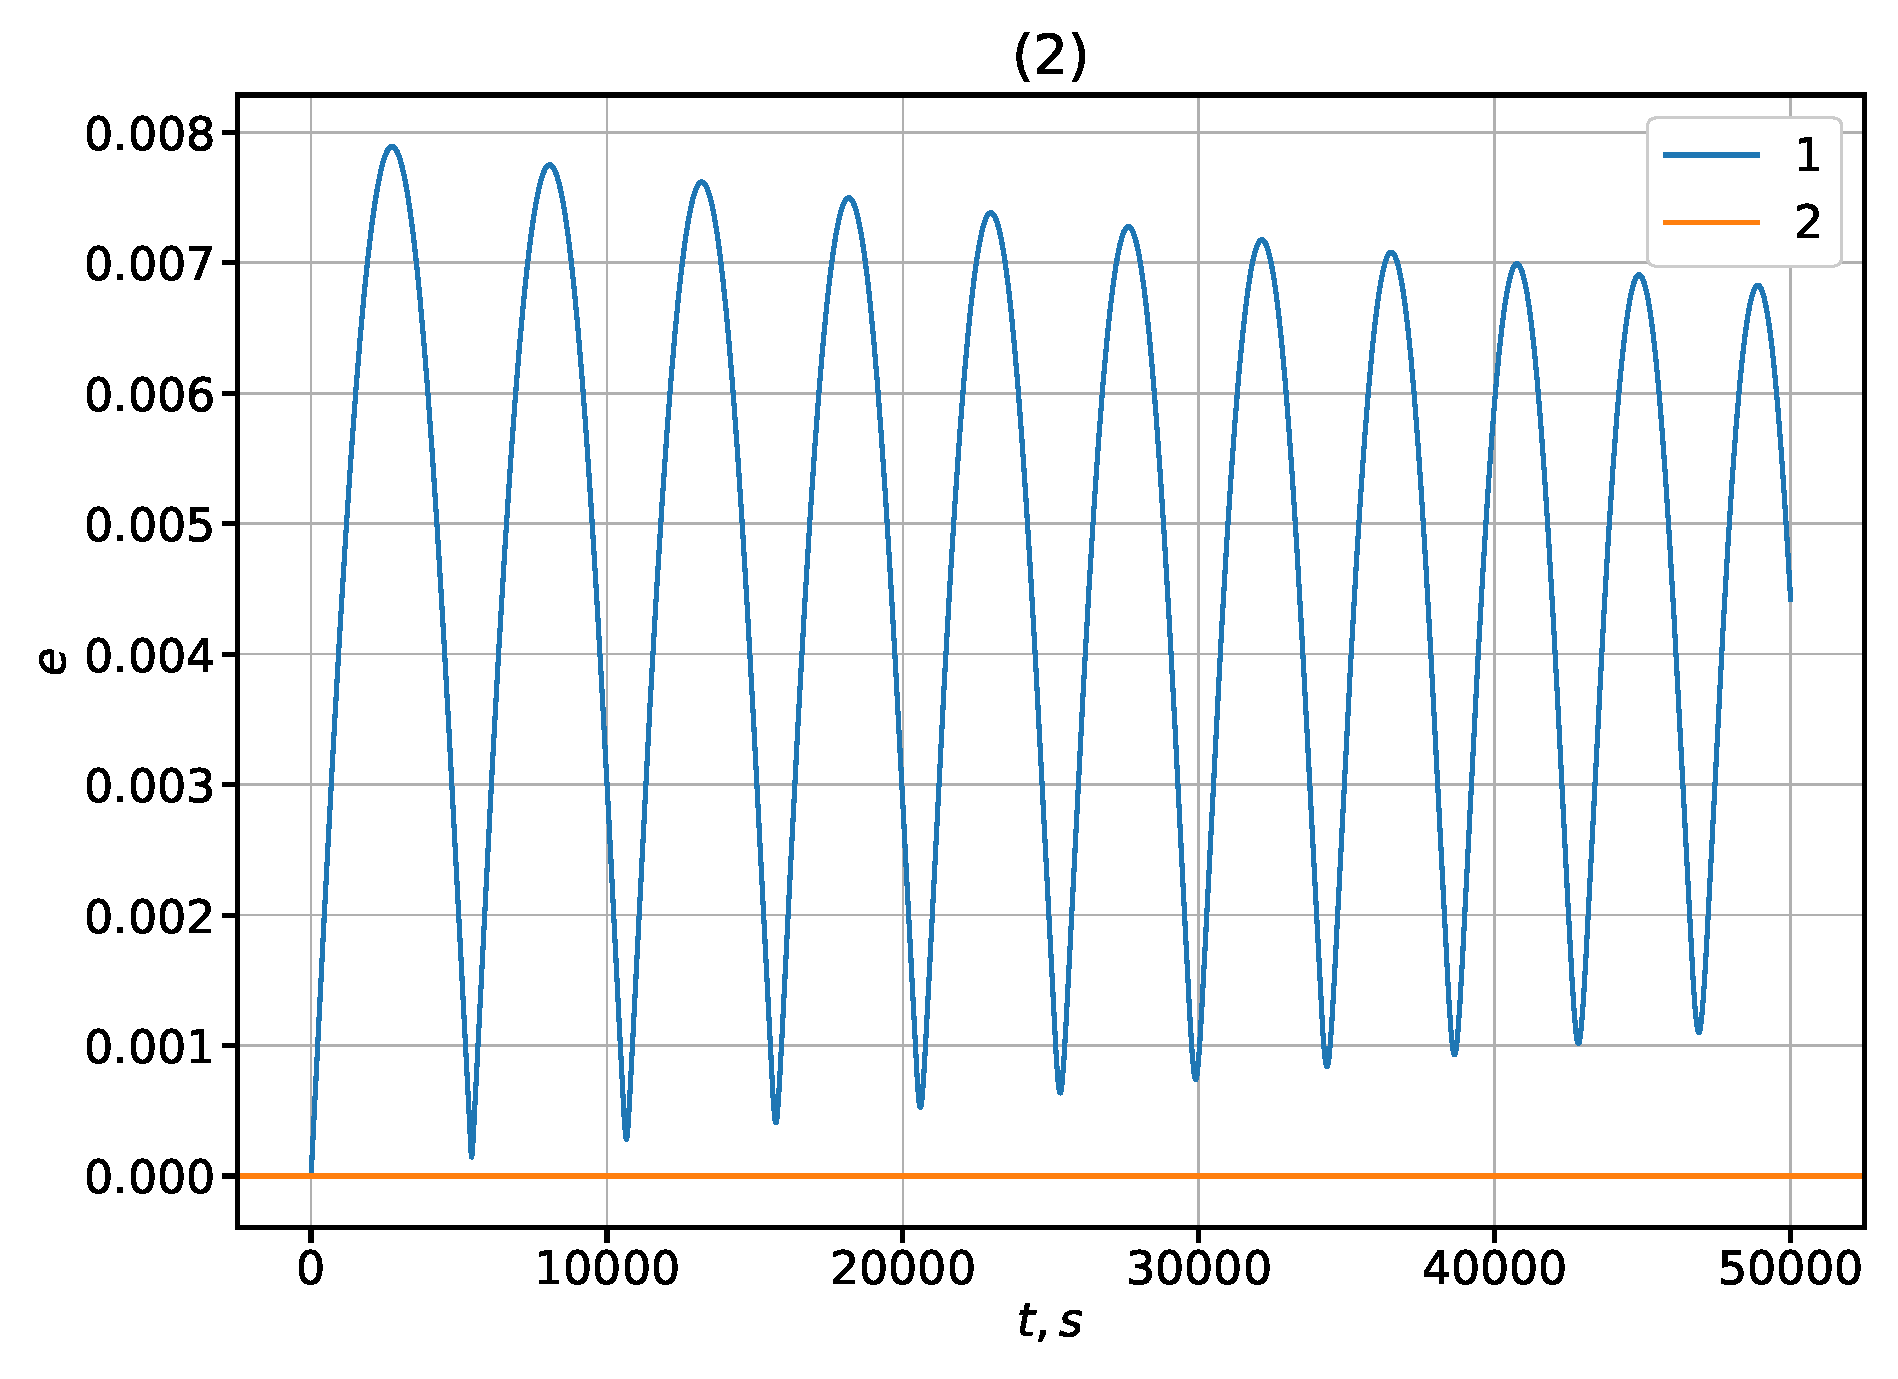
\includegraphics[width=1.0\linewidth]{e_t_2.eps}
    \endminipage\hfill
    \minipage{0.33\textwidth}
      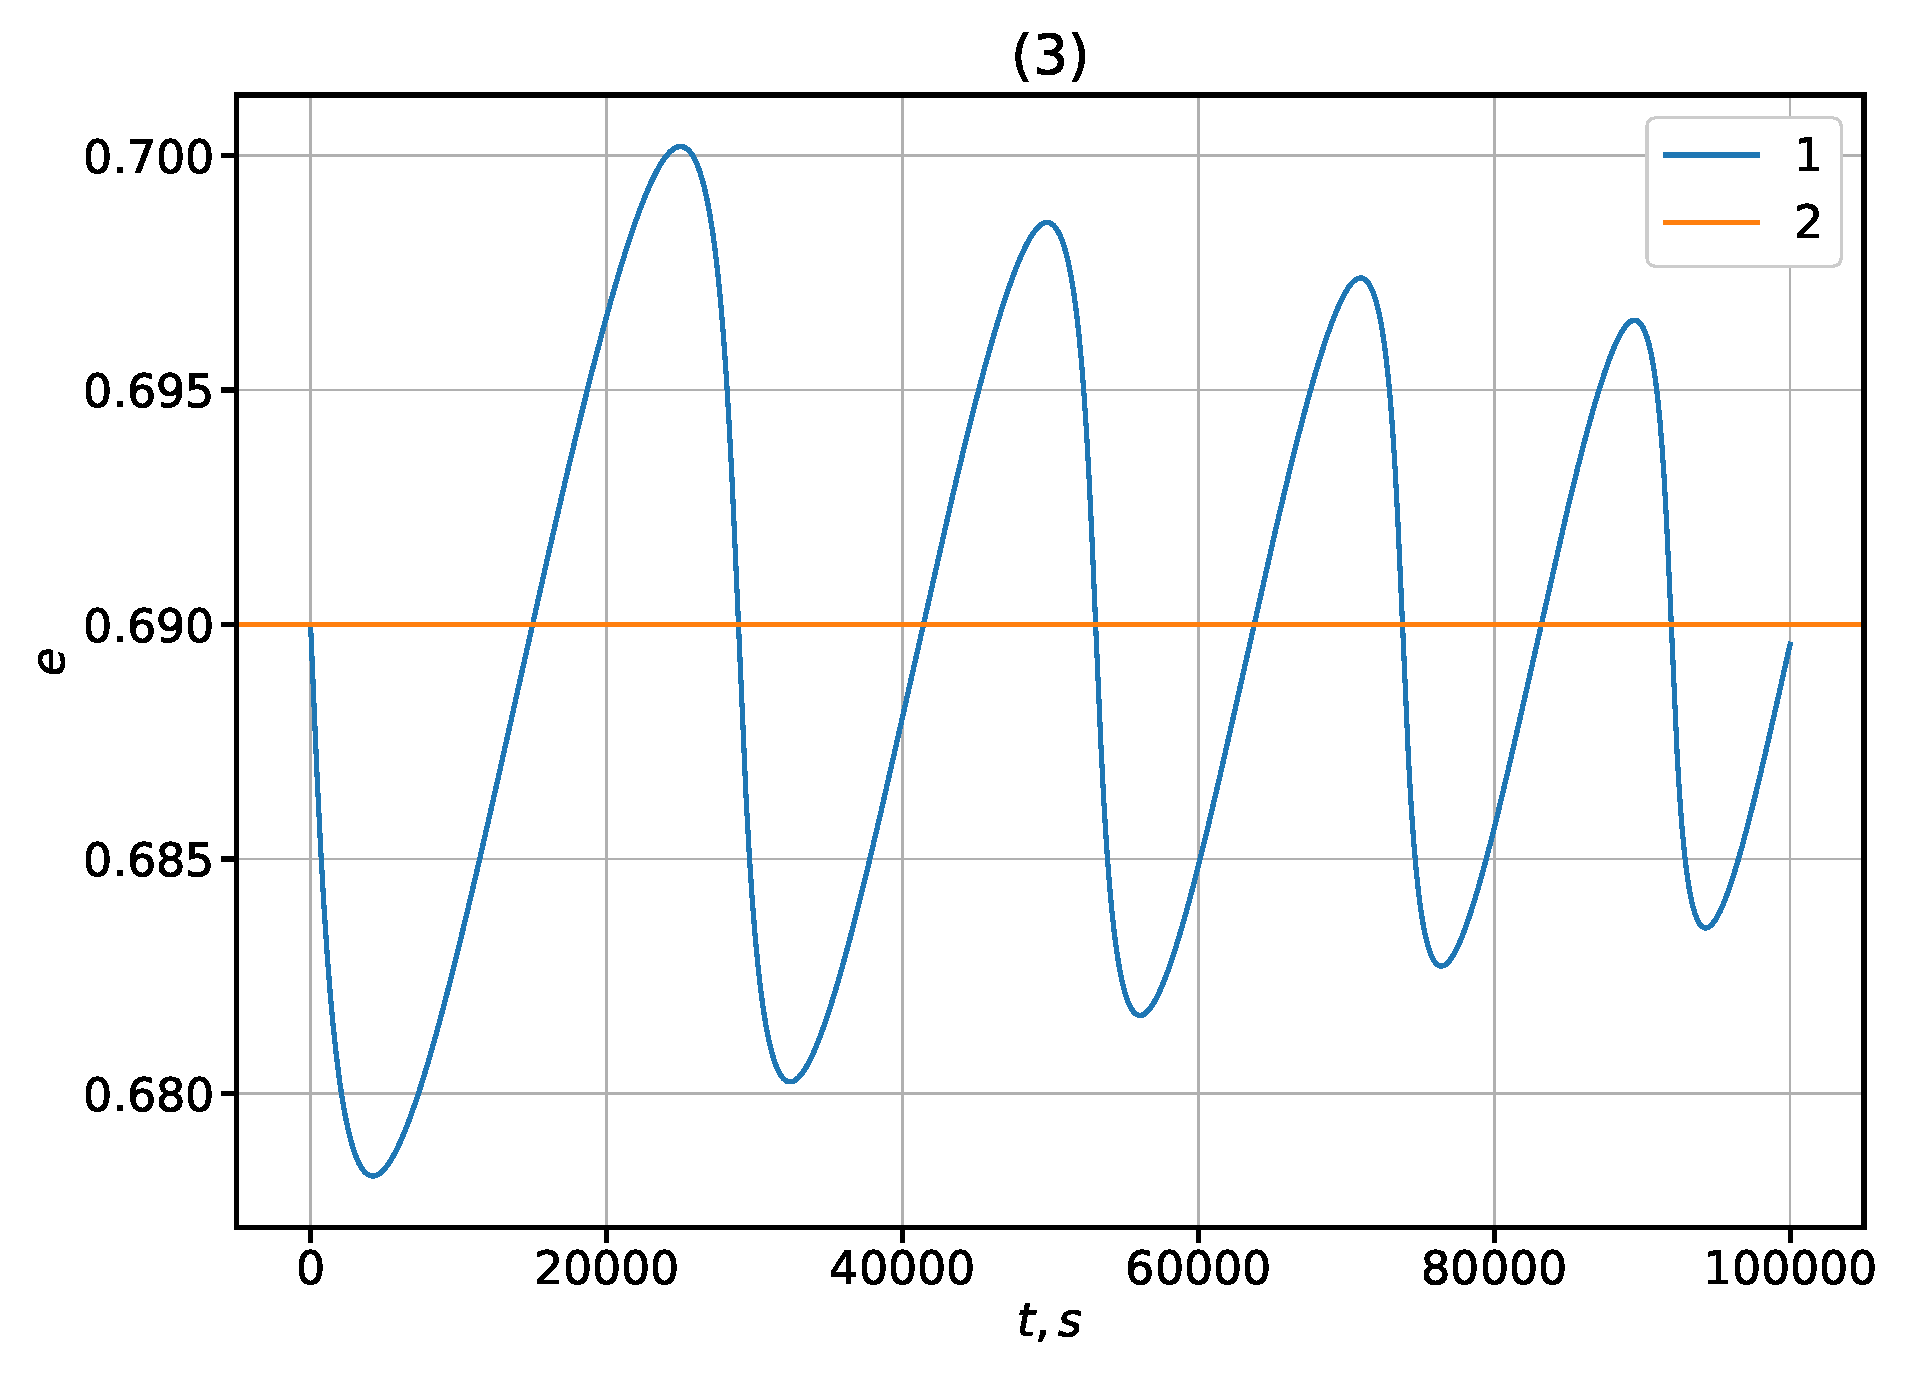
\includegraphics[width=1.0\linewidth]{e_t_3.eps}
    \endminipage
    \caption{Зависимости эксцентреситетов орбит $e$ от времени $t$. 1 - численно рассчитанный эксцентреситет, 
    2 - значение эксцентреситета в начальный момент времени.}
    \label{fig:6}
    \end{figure}

Из графиков траекторий тел на собственных интервалах времени (Рис. \ref{fig:7}) следует независимость формы траектории от времени, что подтверждает
вывод, сделанный из \ref{eq:23}. Однако стоит отметить, что направления орбит не сохраняются, это видно по отмеченным точкам максимального и минимального
отдаления. Это означает, что вектор Лапласа-Рунге-Ленца и в среднем сохраняет свой модуль \ref{fig:6}, но медленно поворачивается.
\begin{figure}[H]
    \minipage{0.33\textwidth}
      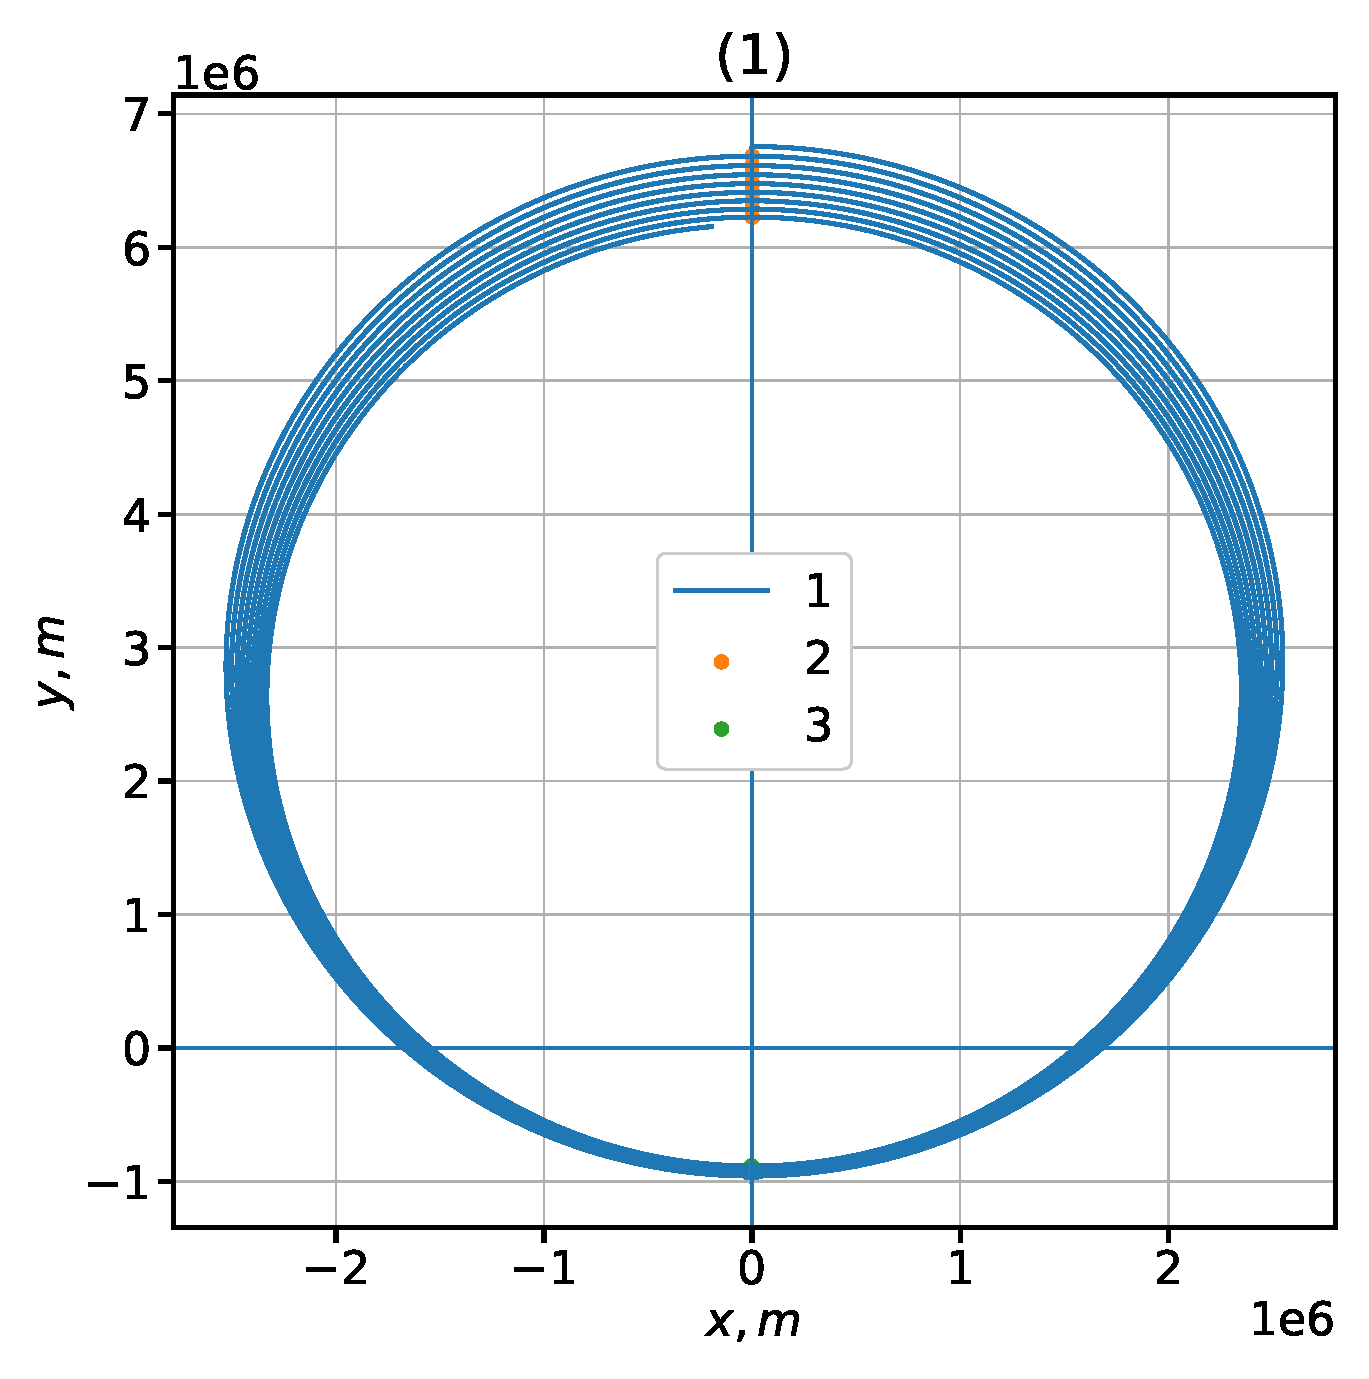
\includegraphics[width=1.0\linewidth]{y_x_1.eps}
    \endminipage\hfill
    \minipage{0.33\textwidth}
      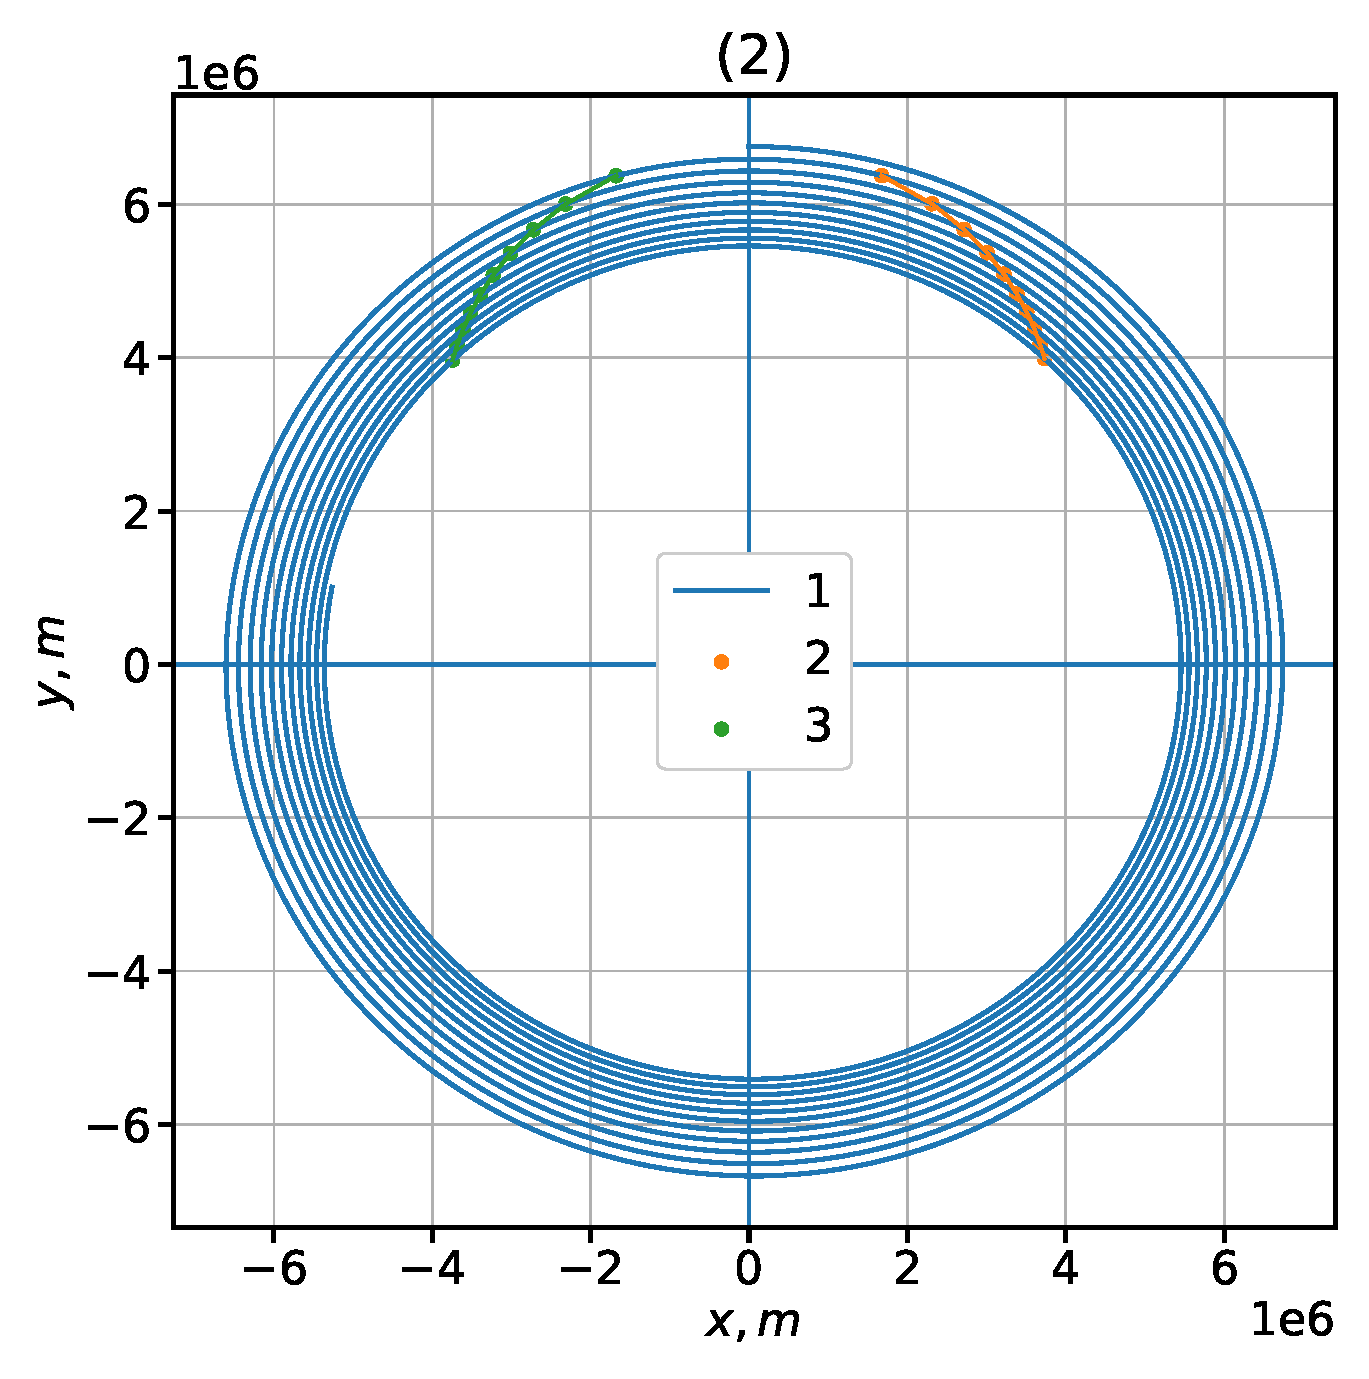
\includegraphics[width=1.0\linewidth]{y_x_2.eps}
    \endminipage\hfill
    \minipage{0.33\textwidth}
      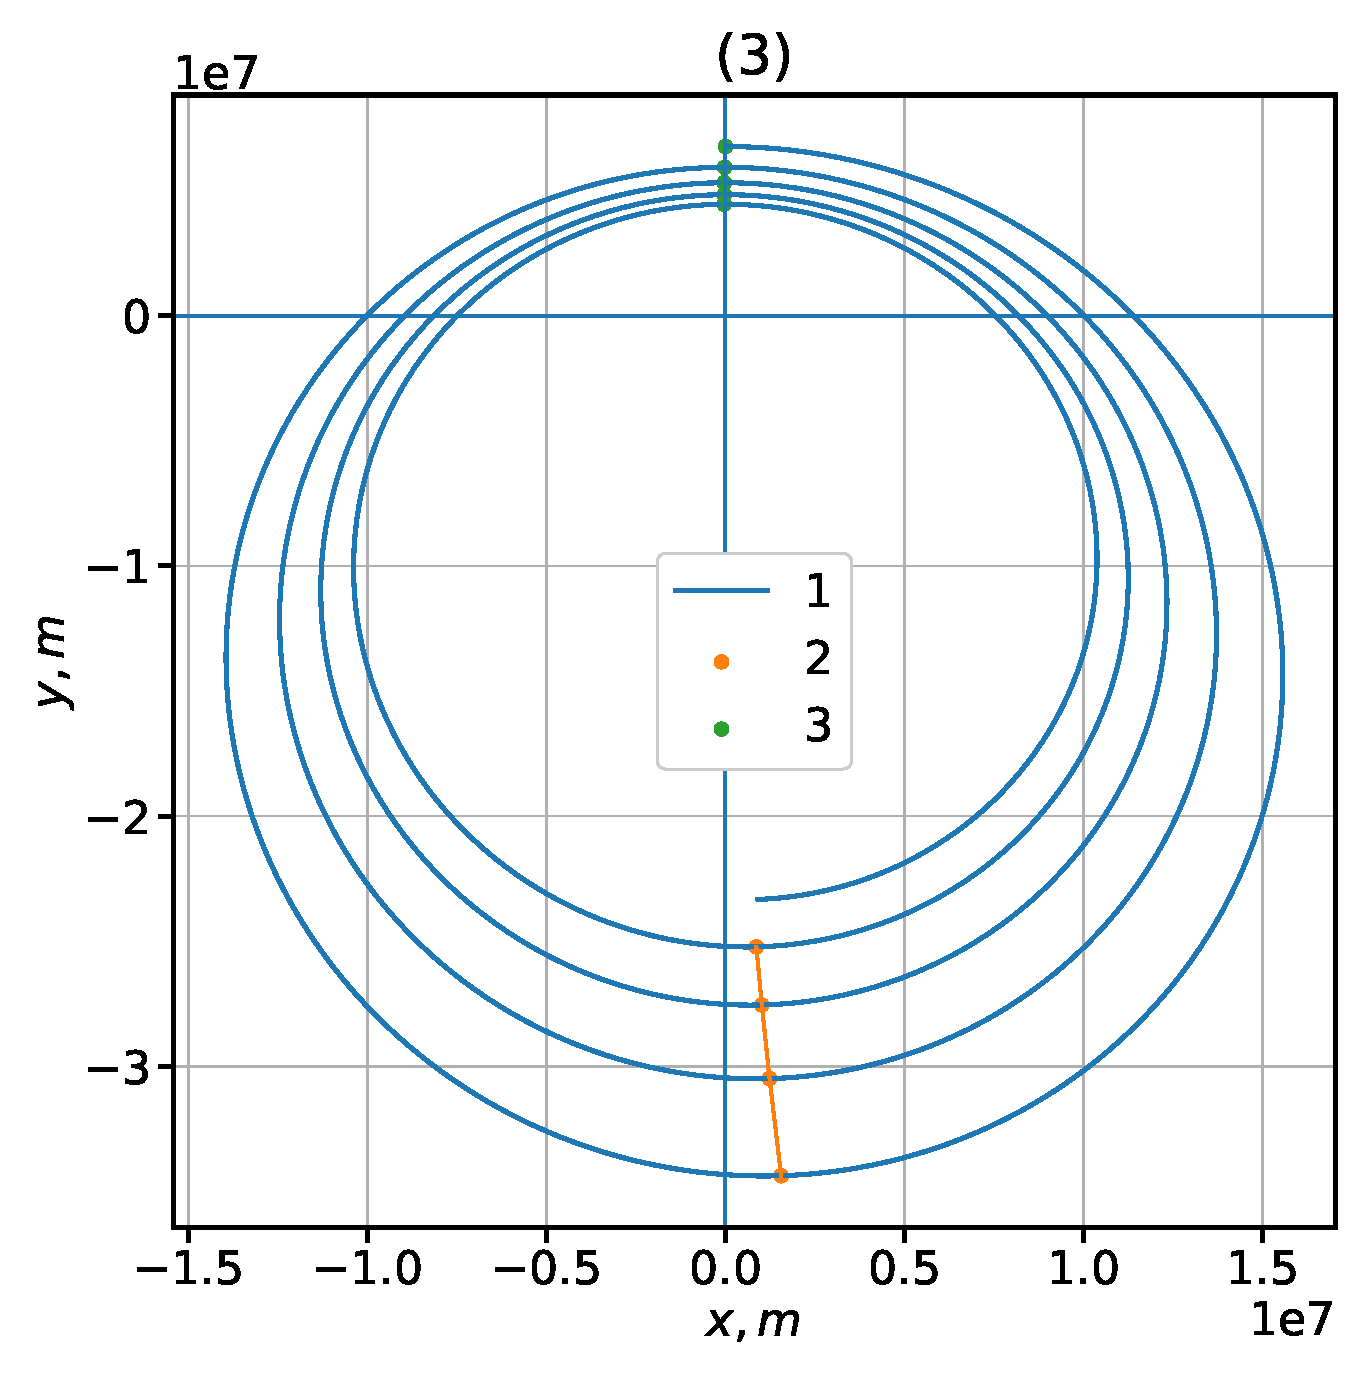
\includegraphics[width=1.0\linewidth]{y_x_3.eps}
    \endminipage
    \caption{Орбиты тел в плоскости их движения. 1 - кривая, являющаяся траекторией движения тела, 
    2 - положения наибольшего удаления тела от центра притяжения, 3 - положения наименьшего удаления тела от центра притяжения.}
    \label{fig:7}
    \end{figure}

Для подтверждения факта поворота орбиты построим графики зависимости угла поворота орбиты от времени (Рис. \ref{fig:8}). В случае изначально
эллиптичных орбит угол отклонения мал, однако для изначально круговой орбиты угол достаточно большой и быстро меняется со временем, можно сказать,
что орбита постоянно вращается для того, чтобы компенсировать свою эллиптичность.
\begin{figure}[H]
    \minipage{0.33\textwidth}
      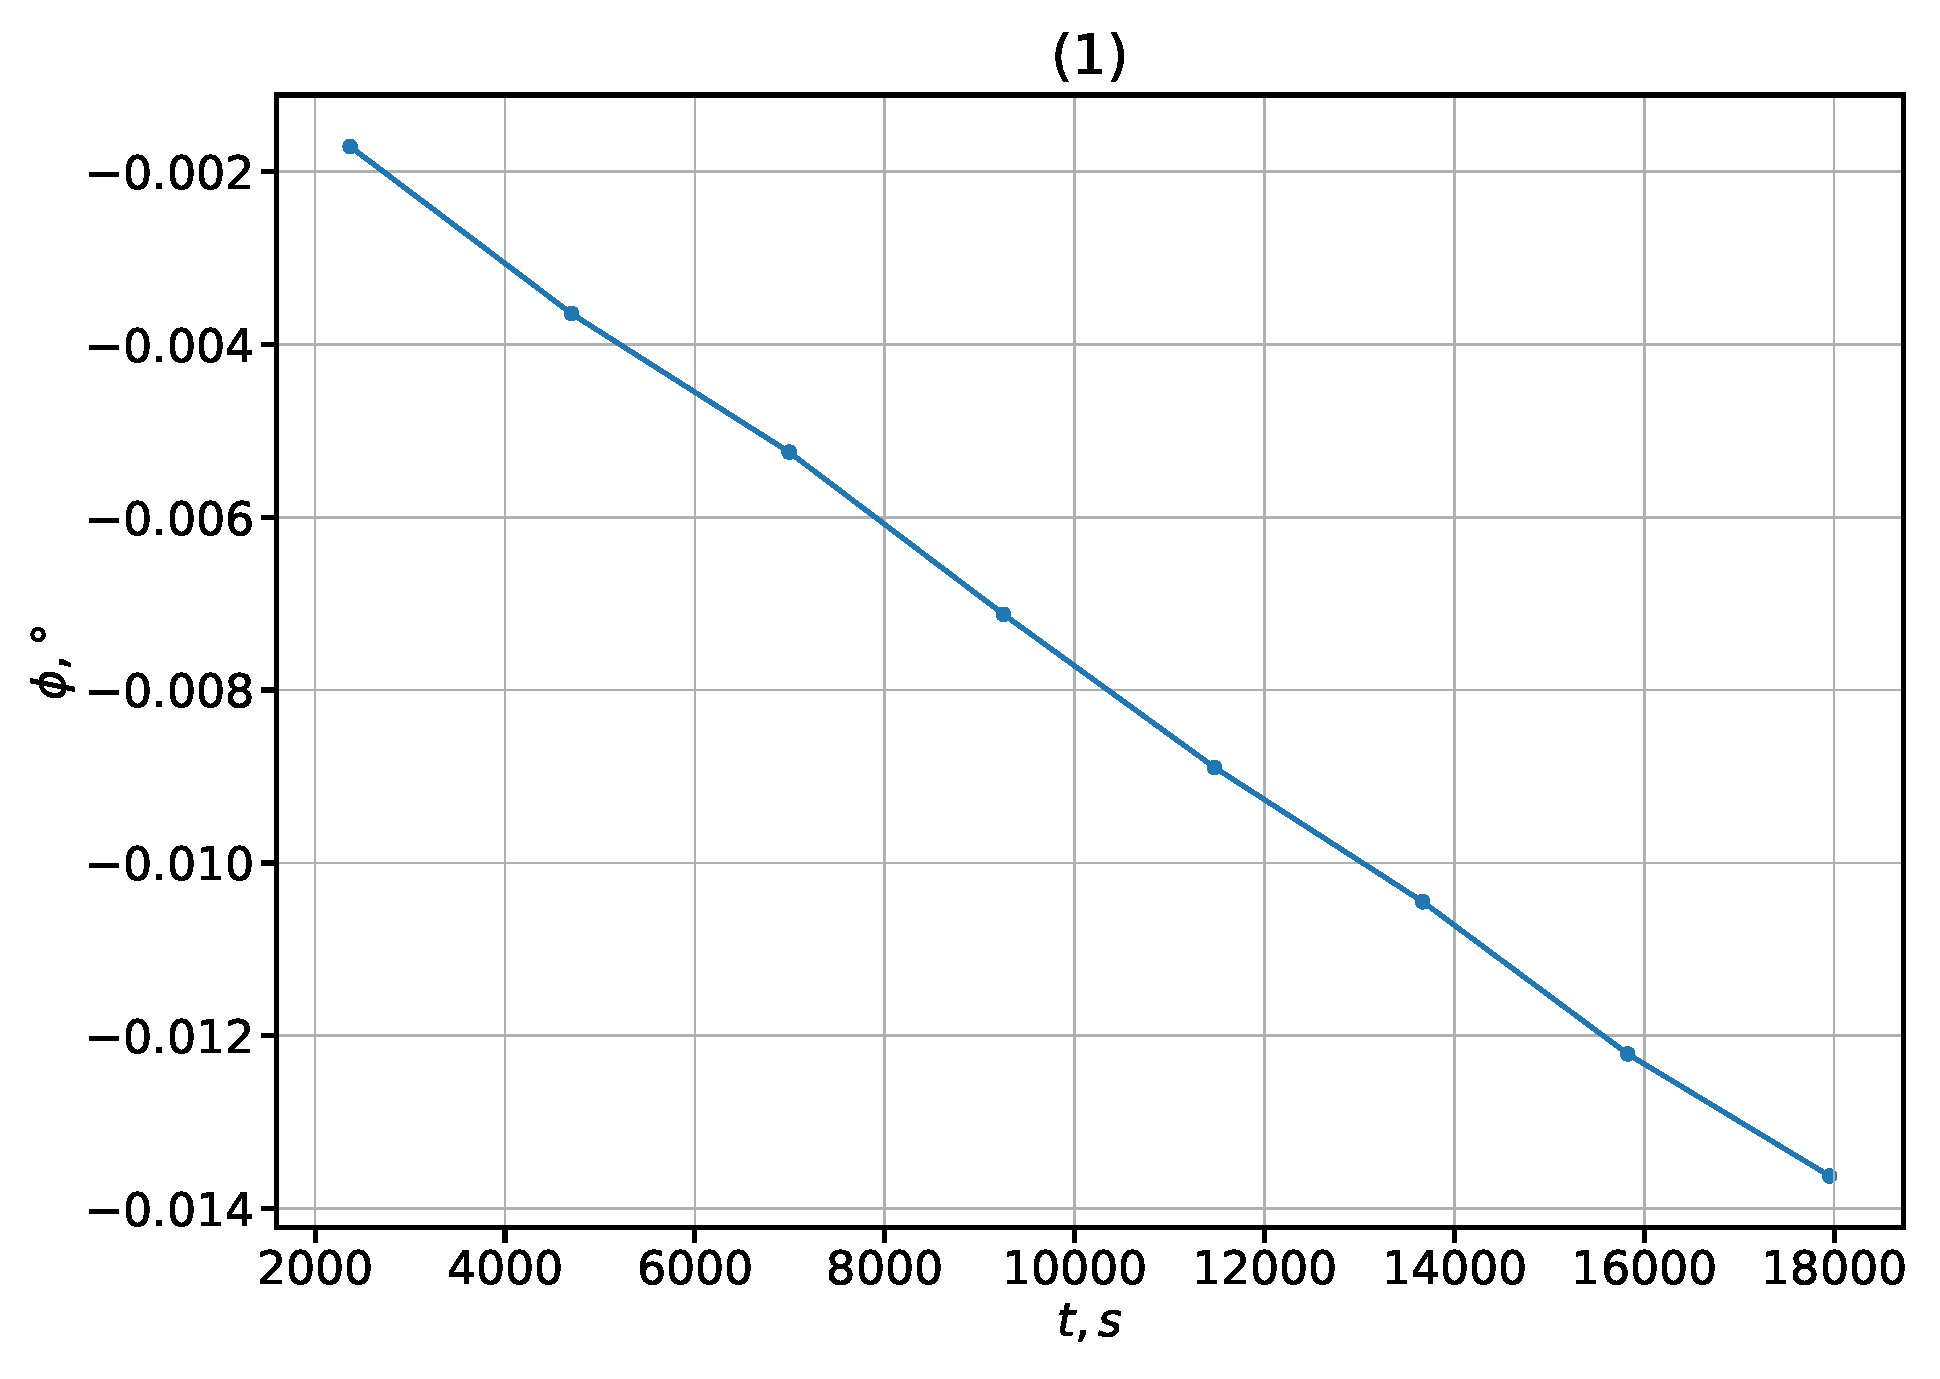
\includegraphics[width=1.0\linewidth]{phi_t_1.eps}
    \endminipage\hfill
    \minipage{0.33\textwidth}
      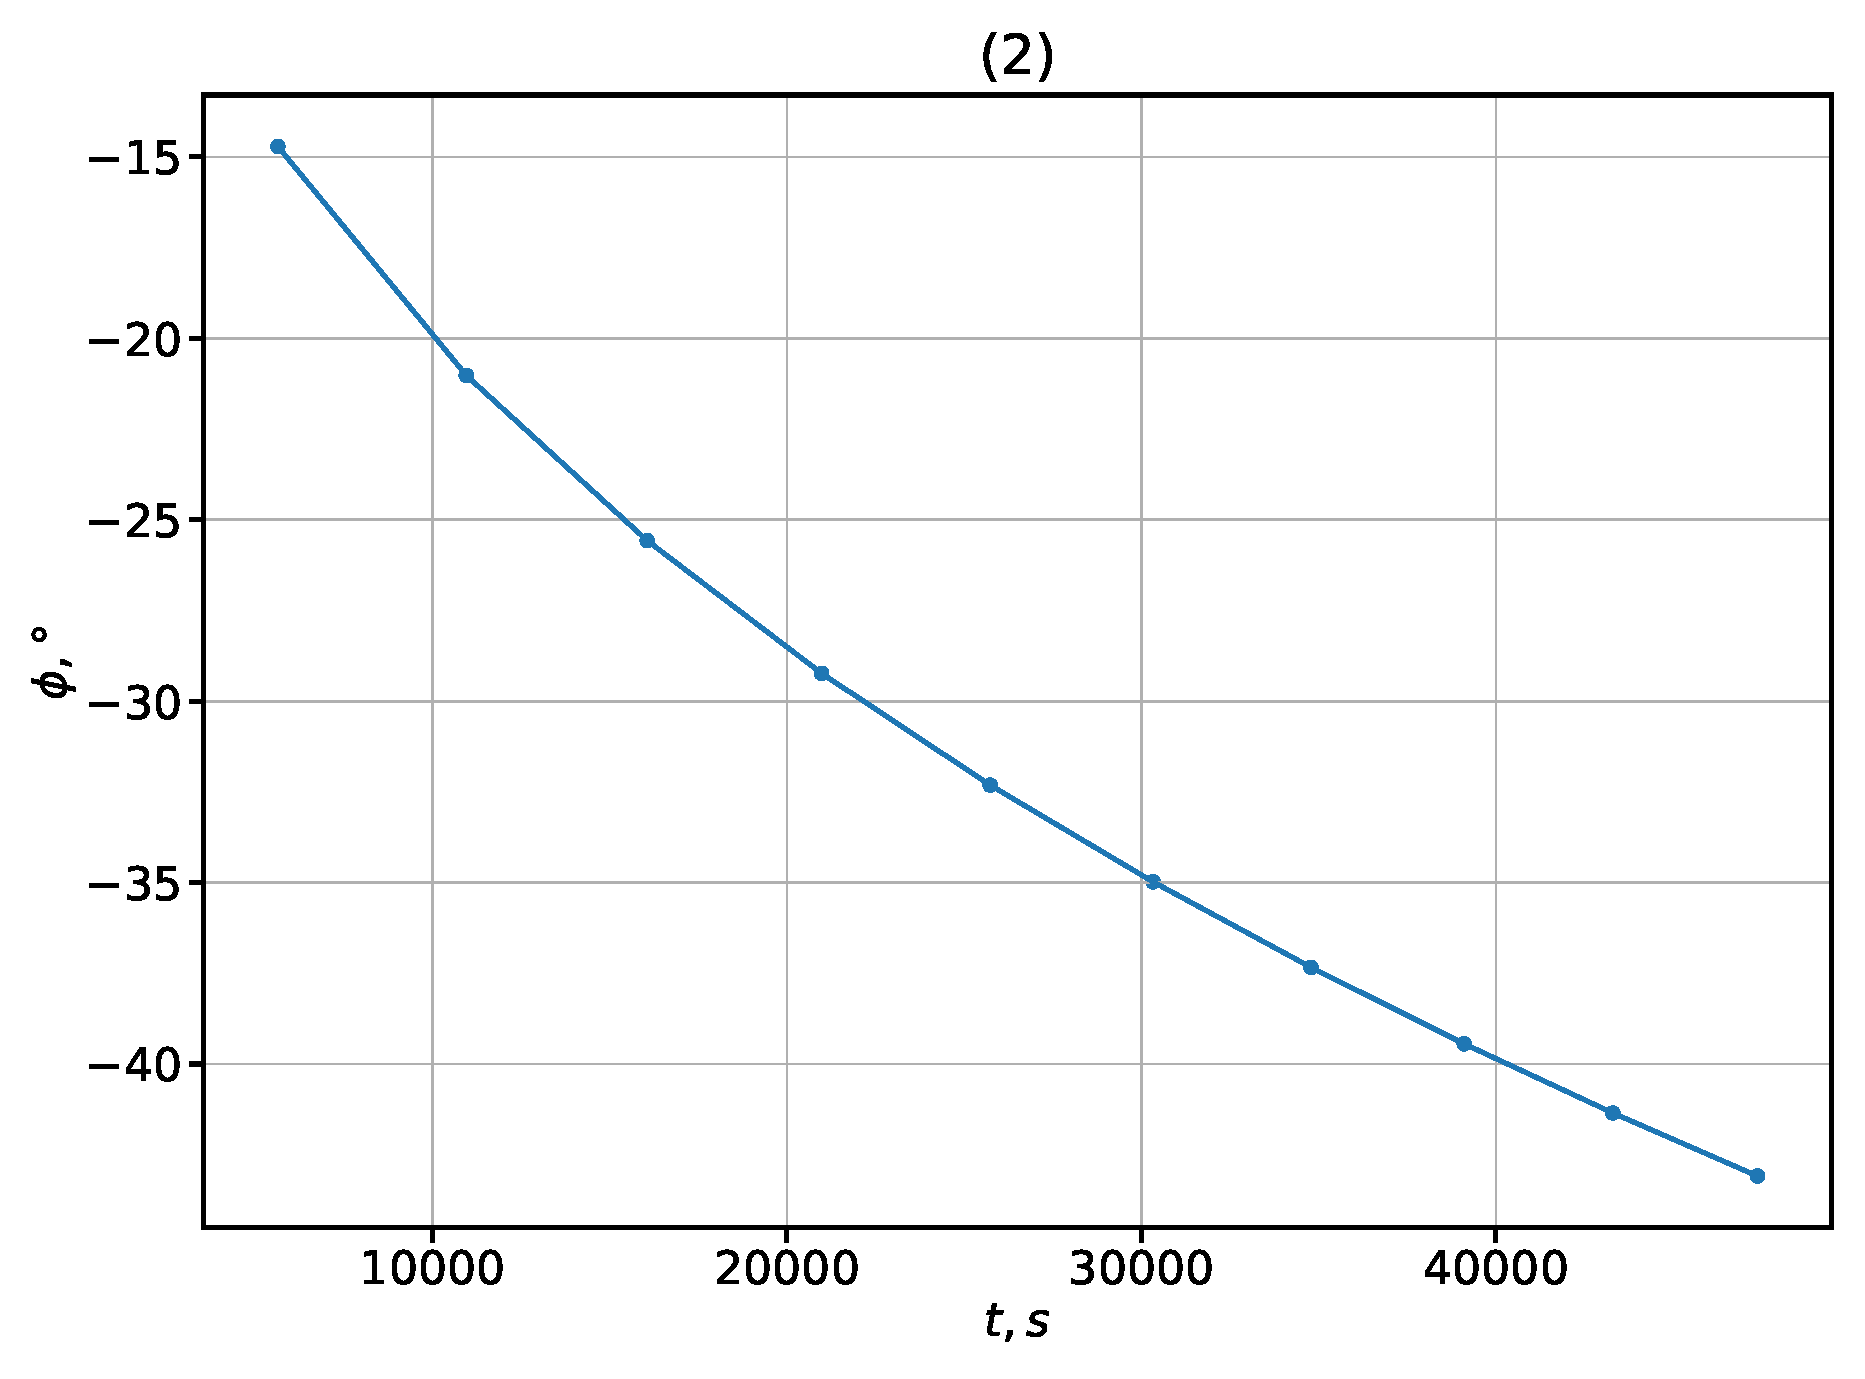
\includegraphics[width=1.0\linewidth]{phi_t_2.eps}
    \endminipage\hfill
    \minipage{0.33\textwidth}
      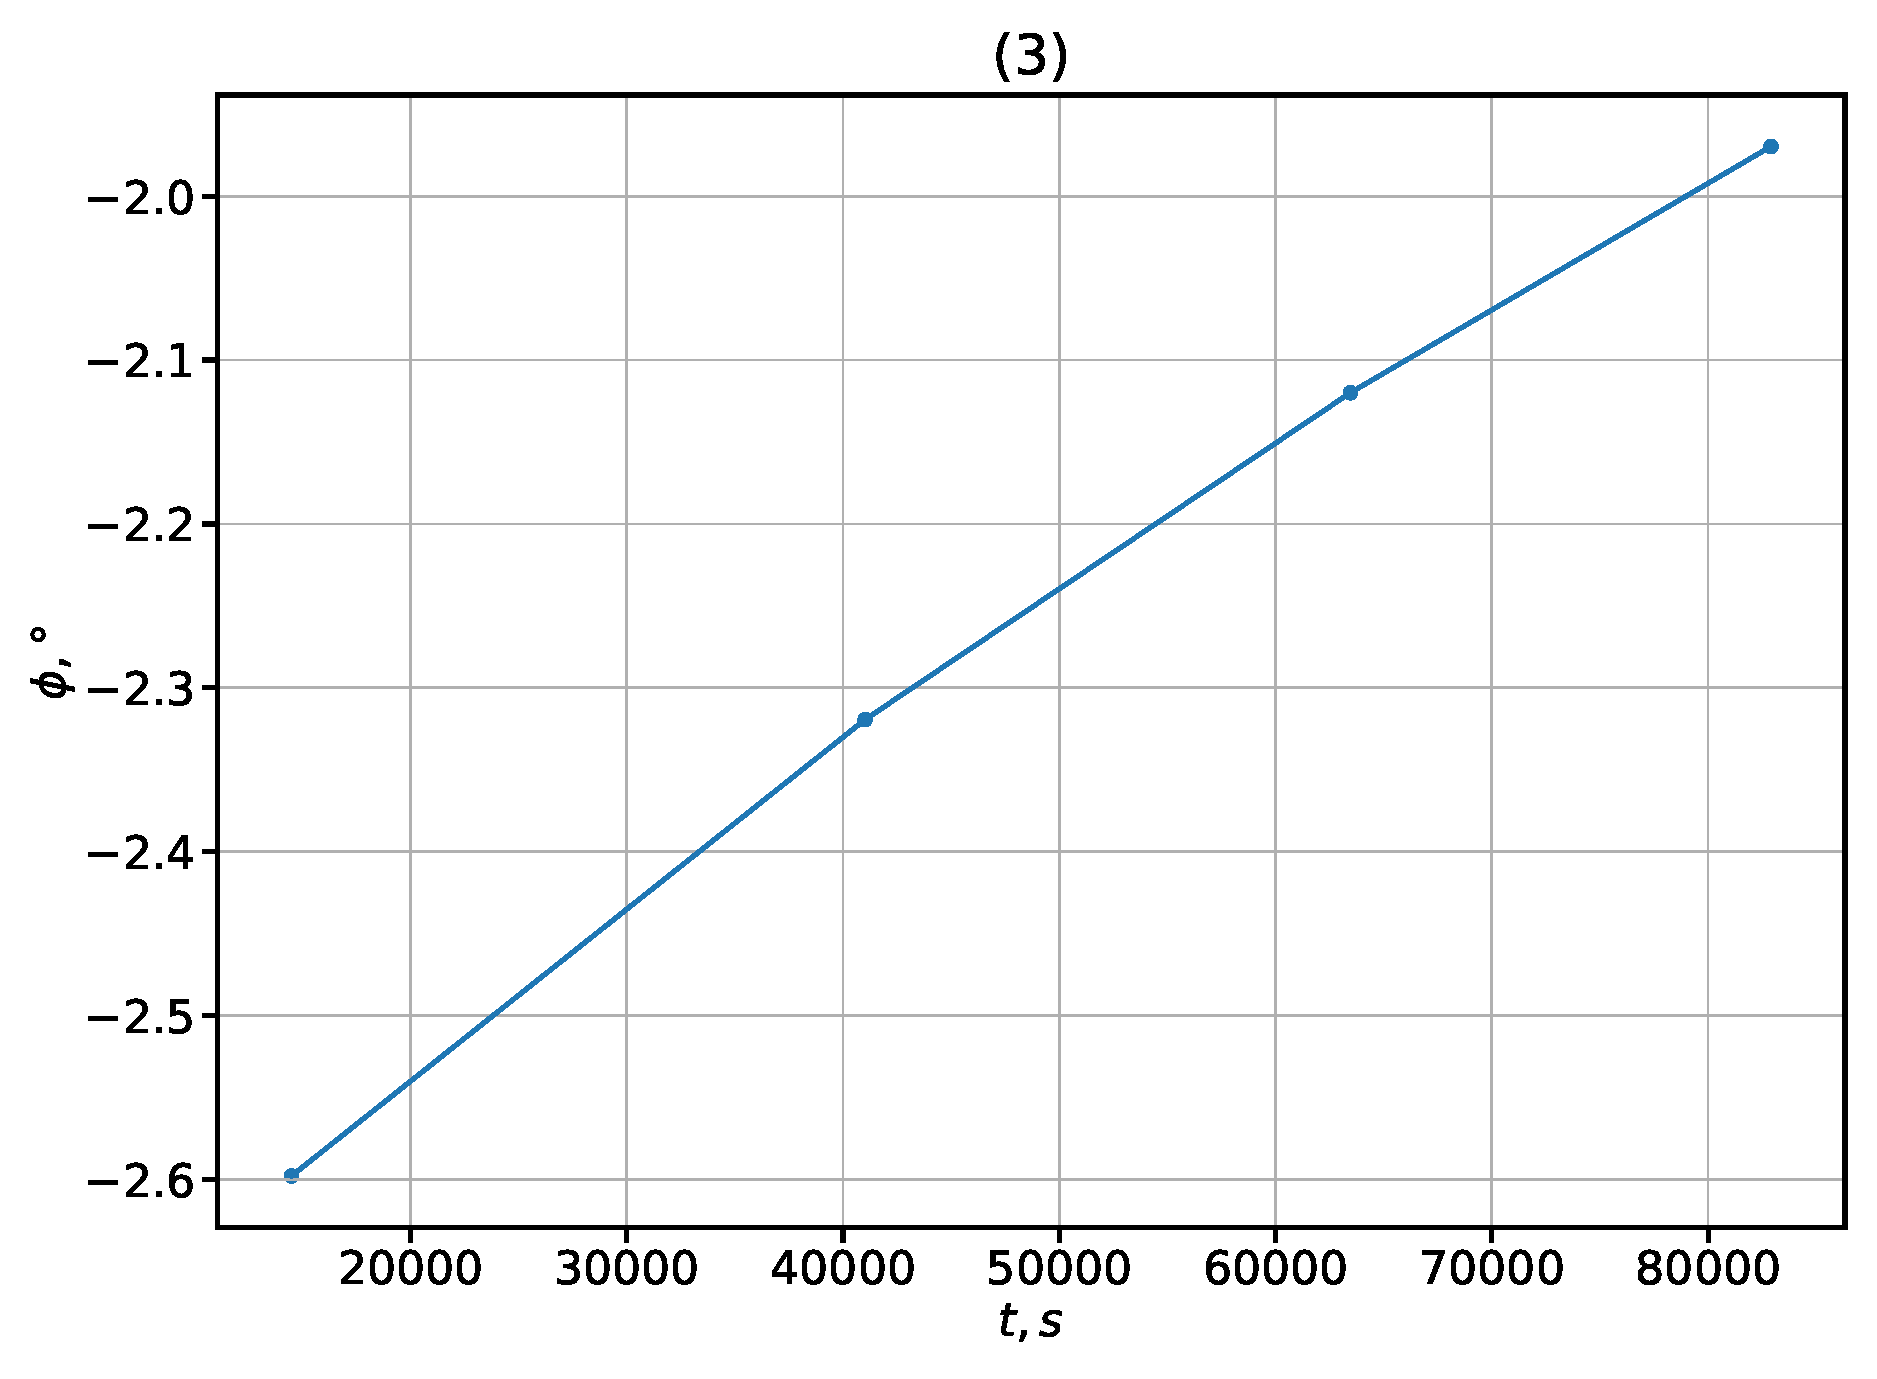
\includegraphics[width=1.0\linewidth]{phi_t_3.eps}
    \endminipage
    \caption{Отклонения направления орбиты $\phi$ от времени $t$.}
    \label{fig:8}
    \end{figure}

\section{Выводы}
Траектория тела, движущегося в гравитационном поле под действием малой силы сопротивления, пропорциональной скорости, будет представлять 
эллипс, с постоянно уменьшающемся фокальным параметром и неизменным эксцентреситетом $r = \frac{p_0e^{-2\gamma t}}{1 + e\cos{\phi}}$.
В случае, если сила сопротивления зависит от скорости в квадрате анализ движения усложняется, однако возможно установить, что 
для тел, двигающихся по близким к круговым орбитам, форма орбиты также сохраняется, однако появляется эллиптичность, эксцентреситет которой
пропорционален коэффиценту силы сопротивления. 

% \section{Использованная литература}
\begin{thebibliography}{9}
    \bibitem{Kvant}
    С. Травин. Ещё раз об аэродинамическом парадоксе. // Квант. - 2011
\end{thebibliography}
% \section{Приложения}

\end{document}